\chapter{Accuracy and computational performance}
\label{chap:performance}

The preceding chapters established the formal order of accuracy, the admissibility of the
discontinuous solutions, and agreement between the three implementations.  This chapter
asks the practical question that motivates Report~2: how much accuracy is obtained for a
given computational cost, and which hardware is best suited to each method?  HLLC is the
authoritative flux throughout the main analysis.  The earlier HLL route is retained only in
a controlled comparison where problem, grid, CFL number, final time, method, and backend
match.

The high-resolution Gaussian fields in Figure~\ref{fig:gaussian-fields-performance}
provide the physical starting point for this analysis. At \(600\times600\), all three HLLC
methods transport the pulse to the same location and preserve a smooth, symmetric field,
while WENO-3 and ADER-3 retain a slightly more compact peak than WENO-2. The remainder
of this chapter quantifies whether that visual improvement justifies the additional
computational cost.

\section{Measurement procedure}

The main smooth campaign uses the periodic two-dimensional Gaussian problem at
\(t=0.1\) and resolutions \(n=25,50,100,200,600\).  WENO-2 and WENO-3 use
\(\mathrm{CFL}=0.4\), while ADER-3 uses its stable smooth value
\(\mathrm{CFL}=0.25\).  OpenMP uses 16 threads.  Each normal campaign point contains a
warm-up followed by repeated measurements. The best repeat is reported because it is least
affected by unrelated activity on the shared Lovelace node.  The speedup of backend \(b\)
is
\begin{equation}
  S_b = \frac{T_{\mathrm{serial}}}{T_b},
  \qquad
  E_{\mathrm{OMP}}(p)=\frac{S_{\mathrm{OMP}}(p)}{p},
  \label{eq:speedup-efficiency}
\end{equation}
Here \(T_{\mathrm{serial}}\) is the serial runtime, \(T_b\) is the runtime of
backend \(b\), and \(S_b\) is that backend's speedup relative to serial.
For OpenMP, \(p\) is the thread count, \(S_{\mathrm{OMP}}(p)\) is the speedup
measured with those \(p\) threads, and \(E_{\mathrm{OMP}}(p)\) is the resulting
parallel efficiency. Thus \(E_{\mathrm{OMP}}=1\) denotes ideal linear scaling.

These method-specific CFL values make the cross-method runtime an end-to-end efficiency
measurement rather than a fixed-time-step kernel benchmark.  In other words, the measured
cost includes the number of updates required by each method in its validated stable
configuration.  Backend speedups remain strictly controlled because all backends use the
same CFL and accepted step count for a given method.  The HLL--HLLC comparison later in
this chapter is stricter still: only rows with matching method, problem, backend, grid,
CFL, final time, and accepted step count are compared.  Consequently, different CFL
numbers are never used to create a favourable backend or flux comparison.

All performance commands use \texttt{--output=none}. Writing the full field to CSV is
therefore excluded.  The outer Python driver times the complete solver process, so the
measurement still contains executable start-up, initialization, the time integration,
terminal diagnostics, and one final error-norm pass for the smooth Gaussian problem.  The
last two costs are small compared with hundreds or thousands of updates at large \(n\), but
they correctly remain visible at the smallest grids.  Accuracy is measured from the same
run using
\begin{equation}
  L_1(\rho)=\frac{1}{N}\sum_{i=1}^{N}
       \left|\rho_i-\rho_i^{\mathrm{exact}}\right|,
  \label{eq:performance-l1}
\end{equation}
where \(N\) is the total number of cells, \(i\) indexes a cell, and
\(\rho_i^{\mathrm{exact}}\) is its exact finite-volume density average. The
corresponding \(L_2\) and \(L_\infty\) norms are retained in the processed data.

The discontinuous campaign uses the quadrant Riemann and shock--bubble problems at
\(t=0.2\), with field output again disabled.  Its main grid sequence is
\(n=50,100,200,600\).  These cases have no smooth exact solution, so their performance is
reported separately from the Gaussian error--runtime comparison.

\section{Smooth accuracy--cost landscape}

Figure~\ref{fig:smooth-runtime-performance} shows the first important change of regime.
At small grids CUDA pays an approximately fixed cost for process and device setup, kernel
launches, and synchronization \cite{nvidia129}, so it is not automatically the fastest backend.  Serial and
OpenMP costs rise much more rapidly with resolution, while the CUDA curves remain shallow
until the device has enough work to amortise those fixed costs.  This is particularly clear
for WENO-2, whose inexpensive spatial operator gives the GPU less arithmetic with which to
hide overhead. The balance between arithmetic work and memory traffic is the central idea of
the roofline performance model \cite{williams2009}.

\begin{figure}[H]
\centering
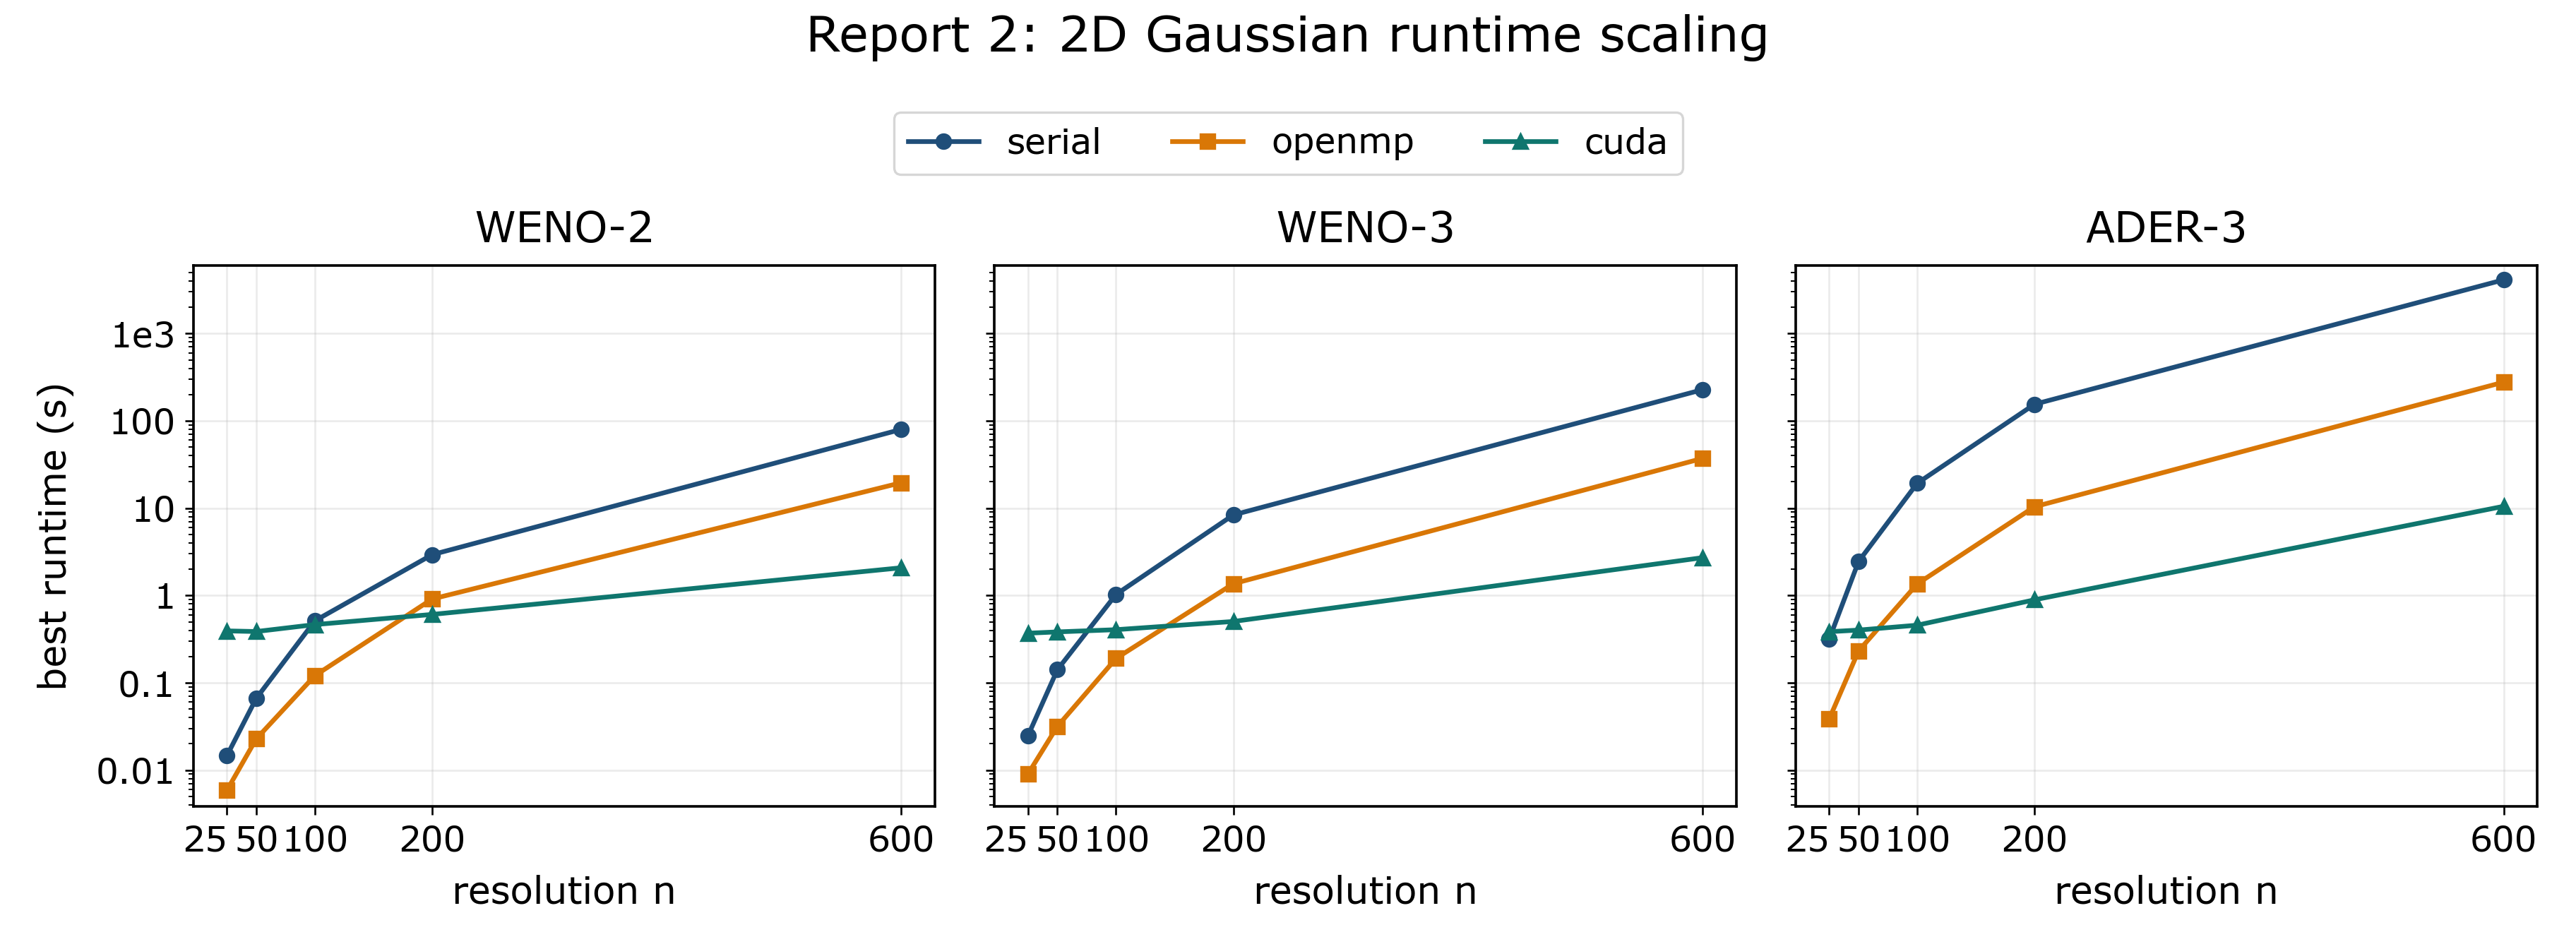
\includegraphics[width=0.98\textwidth]{performance_smooth_runtime_hllc.png}
\caption{HLLC runtime scaling for the smooth two-dimensional Gaussian problem at
\(n=25,50,100,200,600\).  OpenMP uses 16 threads, and field output is disabled during
timing.}
\label{fig:smooth-runtime-performance}
\end{figure}

The same data expressed as speedup are shown in
Figure~\ref{fig:smooth-speedup-performance}.  OpenMP provides a useful but bounded gain:
at \(600^2\) it reaches \(4.08\), \(6.12\), and \(14.86\) for WENO-2, WENO-3, and
ADER-3.  CUDA benefits much more strongly from increasing method complexity, reaching
\(38.43\), \(83.84\), and \(392.01\), respectively.  These numbers do not imply that
ADER-3 is the fastest method.  They show that its much larger serial workload contains
more parallel work and is therefore reduced by a larger factor.

\begin{figure}[H]
\centering
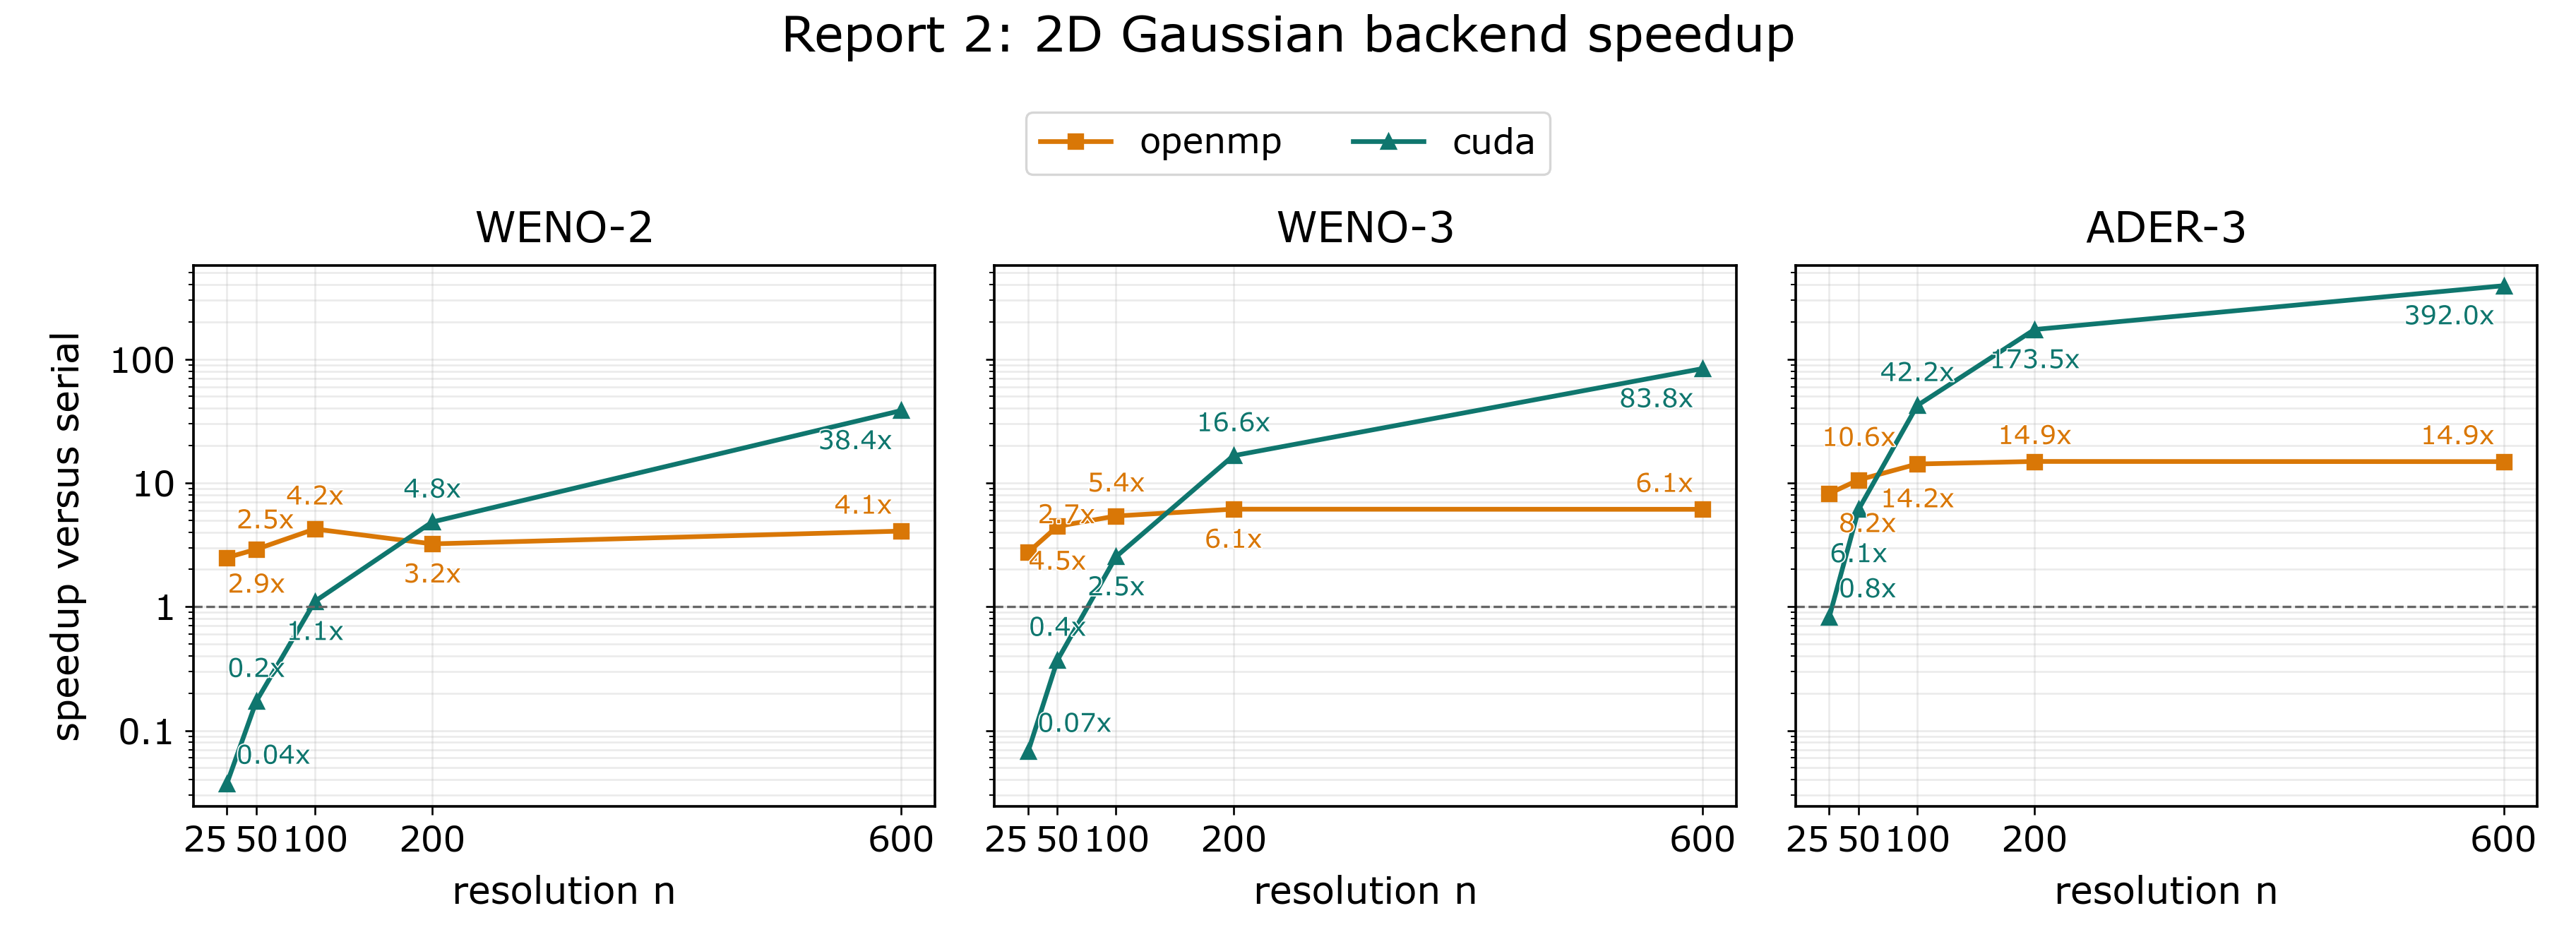
\includegraphics[width=0.98\textwidth]{performance_smooth_speedup_hllc.png}
\caption{HLLC backend speedup relative to serial for the smooth Gaussian campaign at
\(n=25,50,100,200,600\).  OpenMP uses 16 threads.}
\label{fig:smooth-speedup-performance}
\end{figure}

Table~\ref{tab:smooth-n600-performance} combines cost and accuracy at the largest common
all-backend grid.  WENO-3 and ADER-3 reduce the WENO-2 density error by factors of
approximately 27.2 and 28.0.  On serial CPU this accuracy is expensive: ADER-3 takes more
than \(4.1\times10^3\) seconds.  CUDA changes the ranking.  WENO-3 requires only 2.71 s,
close to the 2.08 s WENO-2 run, while retaining its much lower error.  ADER-3 reaches almost
the same error as WENO-3 but takes 10.51 s.  WENO-3 is therefore the strongest measured
accuracy--runtime compromise at \(600^2\). ADER-3 demonstrates the desired order and large
parallel speedup, but its one-step predictor is not yet cost competitive.

\begin{table}[H]
\centering
\small
\begin{tabular}{lrrrrrr}
\toprule
Method & \(L_1(\rho)\) & Serial & OpenMP & CUDA & OMP sp. & CUDA sp. \\
\midrule
WENO-2 & \(4.703\times10^{-7}\) & 79.86 & 19.56 & 2.08 & 4.08 & 38.43 \\
WENO-3 & \(1.726\times10^{-8}\) & 227.31 & 37.13 & 2.71 & 6.12 & 83.84 \\
ADER-3 & \(1.681\times10^{-8}\) & 4118.48 & 277.20 & 10.51 & 14.86 & 392.01 \\
\bottomrule
\end{tabular}
\caption{Smooth HLLC results at \(600\times600\) on Lovelace A30.  Times are best
repeated wall-clock measurements in seconds.}
\label{tab:smooth-n600-performance}
\end{table}

Figure~\ref{fig:smooth-tradeoff-performance} presents the full grid sequence directly in
accuracy--runtime space.  Moving down means lower error and moving left means lower cost.
The error for a fixed method and resolution is essentially backend independent after the
consistency checks in Chapter~\ref{chap:backend-consistency}. Changing backend therefore
moves a point horizontally.  This is why groups of serial, OpenMP, and CUDA points lie on
the same error level.  CUDA shifts the third-order methods far enough left that their
accuracy advantage becomes practical rather than merely formal.

\begin{figure}[H]
\centering
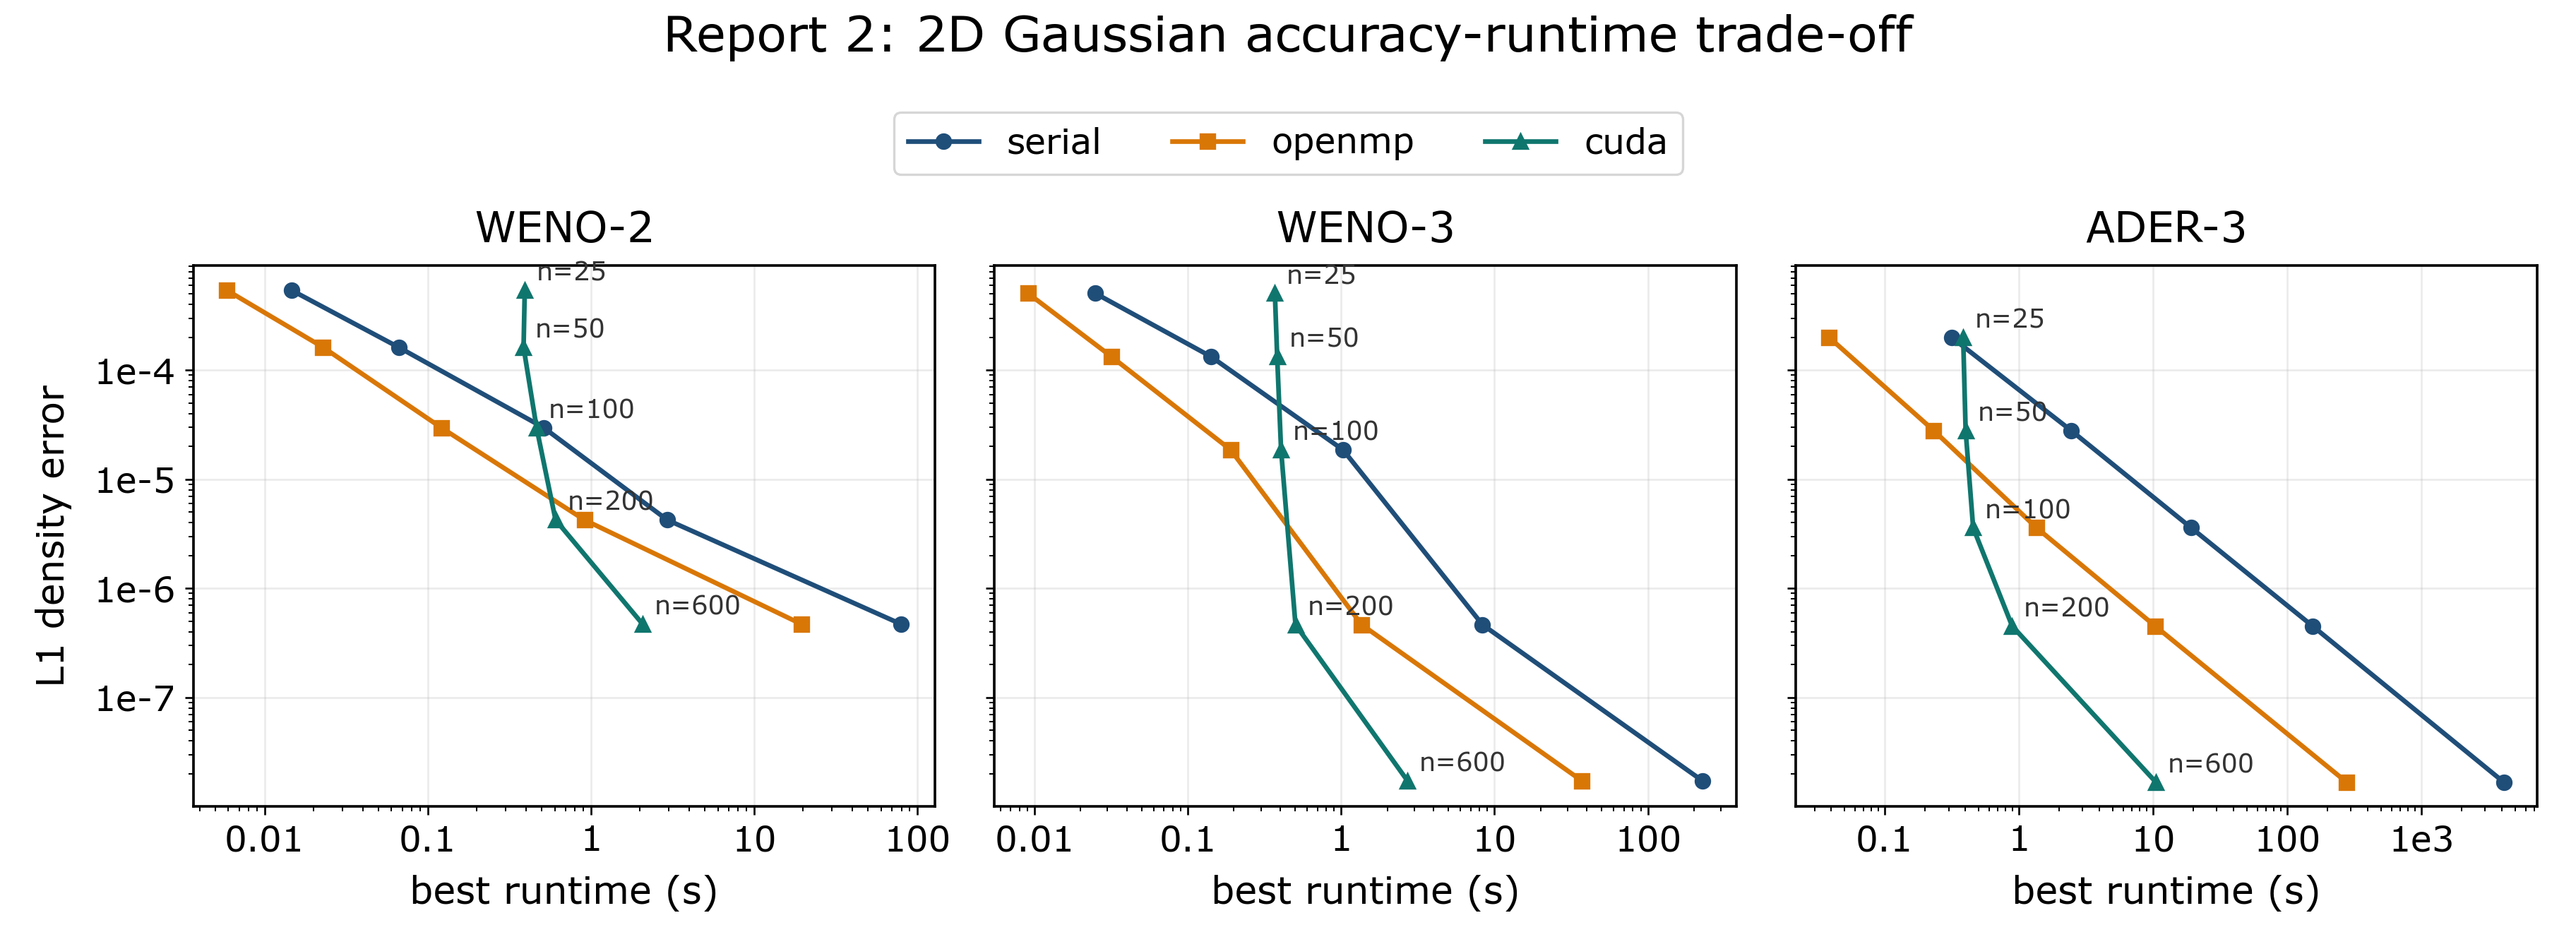
\includegraphics[width=0.96\textwidth]{performance_smooth_accuracy_runtime_hllc.png}
\caption{HLLC density-error versus runtime for the smooth Gaussian campaign.}
\label{fig:smooth-tradeoff-performance}
\end{figure}

The conclusion is not simply that higher order is better.  WENO-2 remains attractive for
small or latency-dominated calculations, where the target error is modest.  WENO-3 becomes
preferable as resolution and accuracy requirements increase.  ADER-3 offers comparable
third-order error but currently requires substantially more work per cell, so its value
depends on whether future kernel and predictor optimization can close that cost gap.

\section{Performance on discontinuous problems}

The two discontinuous cases test whether the smooth conclusions survive when HLLC branch
selection, positivity checks, and local fallback are active.  Table~\ref{tab:discontinuous-n600}
shows the \(600^2\) endpoint.  CUDA remains decisive: speedups range from 48.57 to 478.53
for the quadrant problem and from 84.98 to 427.15 for shock--bubble.  The larger ADER-3
speedups again arise from a very expensive serial baseline, not from a lower absolute cost.
Its CUDA runs remain slower than either WENO method.

\begin{table}[H]
\centering
\small
\begin{tabular}{llrrrrr}
\toprule
Case & Method & Serial & OpenMP & CUDA & OMP sp. & CUDA sp. \\
\midrule
Quadrant & WENO-2 & 388.55 & 95.18 & 8.00 & 4.08 & 48.57 \\
Quadrant & WENO-3 & 1153.71 & 197.29 & 11.86 & 5.85 & 97.24 \\
Quadrant & ADER-3 & 21749.43 & 1941.68 & 45.45 & 11.20 & 478.53 \\
Shock--bubble & WENO-2 & 741.91 & 173.33 & 8.54 & 4.28 & 86.89 \\
Shock--bubble & WENO-3 & 2067.88 & 356.72 & 24.33 & 5.80 & 84.98 \\
Shock--bubble & ADER-3 & 36977.24 & 2496.39 & 86.57 & 14.81 & 427.15 \\
\bottomrule
\end{tabular}
\caption{HLLC discontinuous timing at \(600\times600\).  The selected stable CFL values
are 0.2 for both WENO methods and 0.14 for ADER-3.}
\label{tab:discontinuous-n600}
\end{table}

The absolute CUDA costs qualify these speedups. In the quadrant case, WENO-3 costs
1.48 times WENO-2 and ADER-3 costs 3.83 times WENO-3. The corresponding shock--bubble
ratios are 2.85 and 3.56. WENO-3 therefore buys cleaner contact resolution at a moderate
cost, whereas much of ADER-3's extra predictor work is lost near shocks when the robust
fallback is activated. Its large speedup reflects abundant parallel work, not the lowest
time to solution.

\begin{figure}[H]
\centering
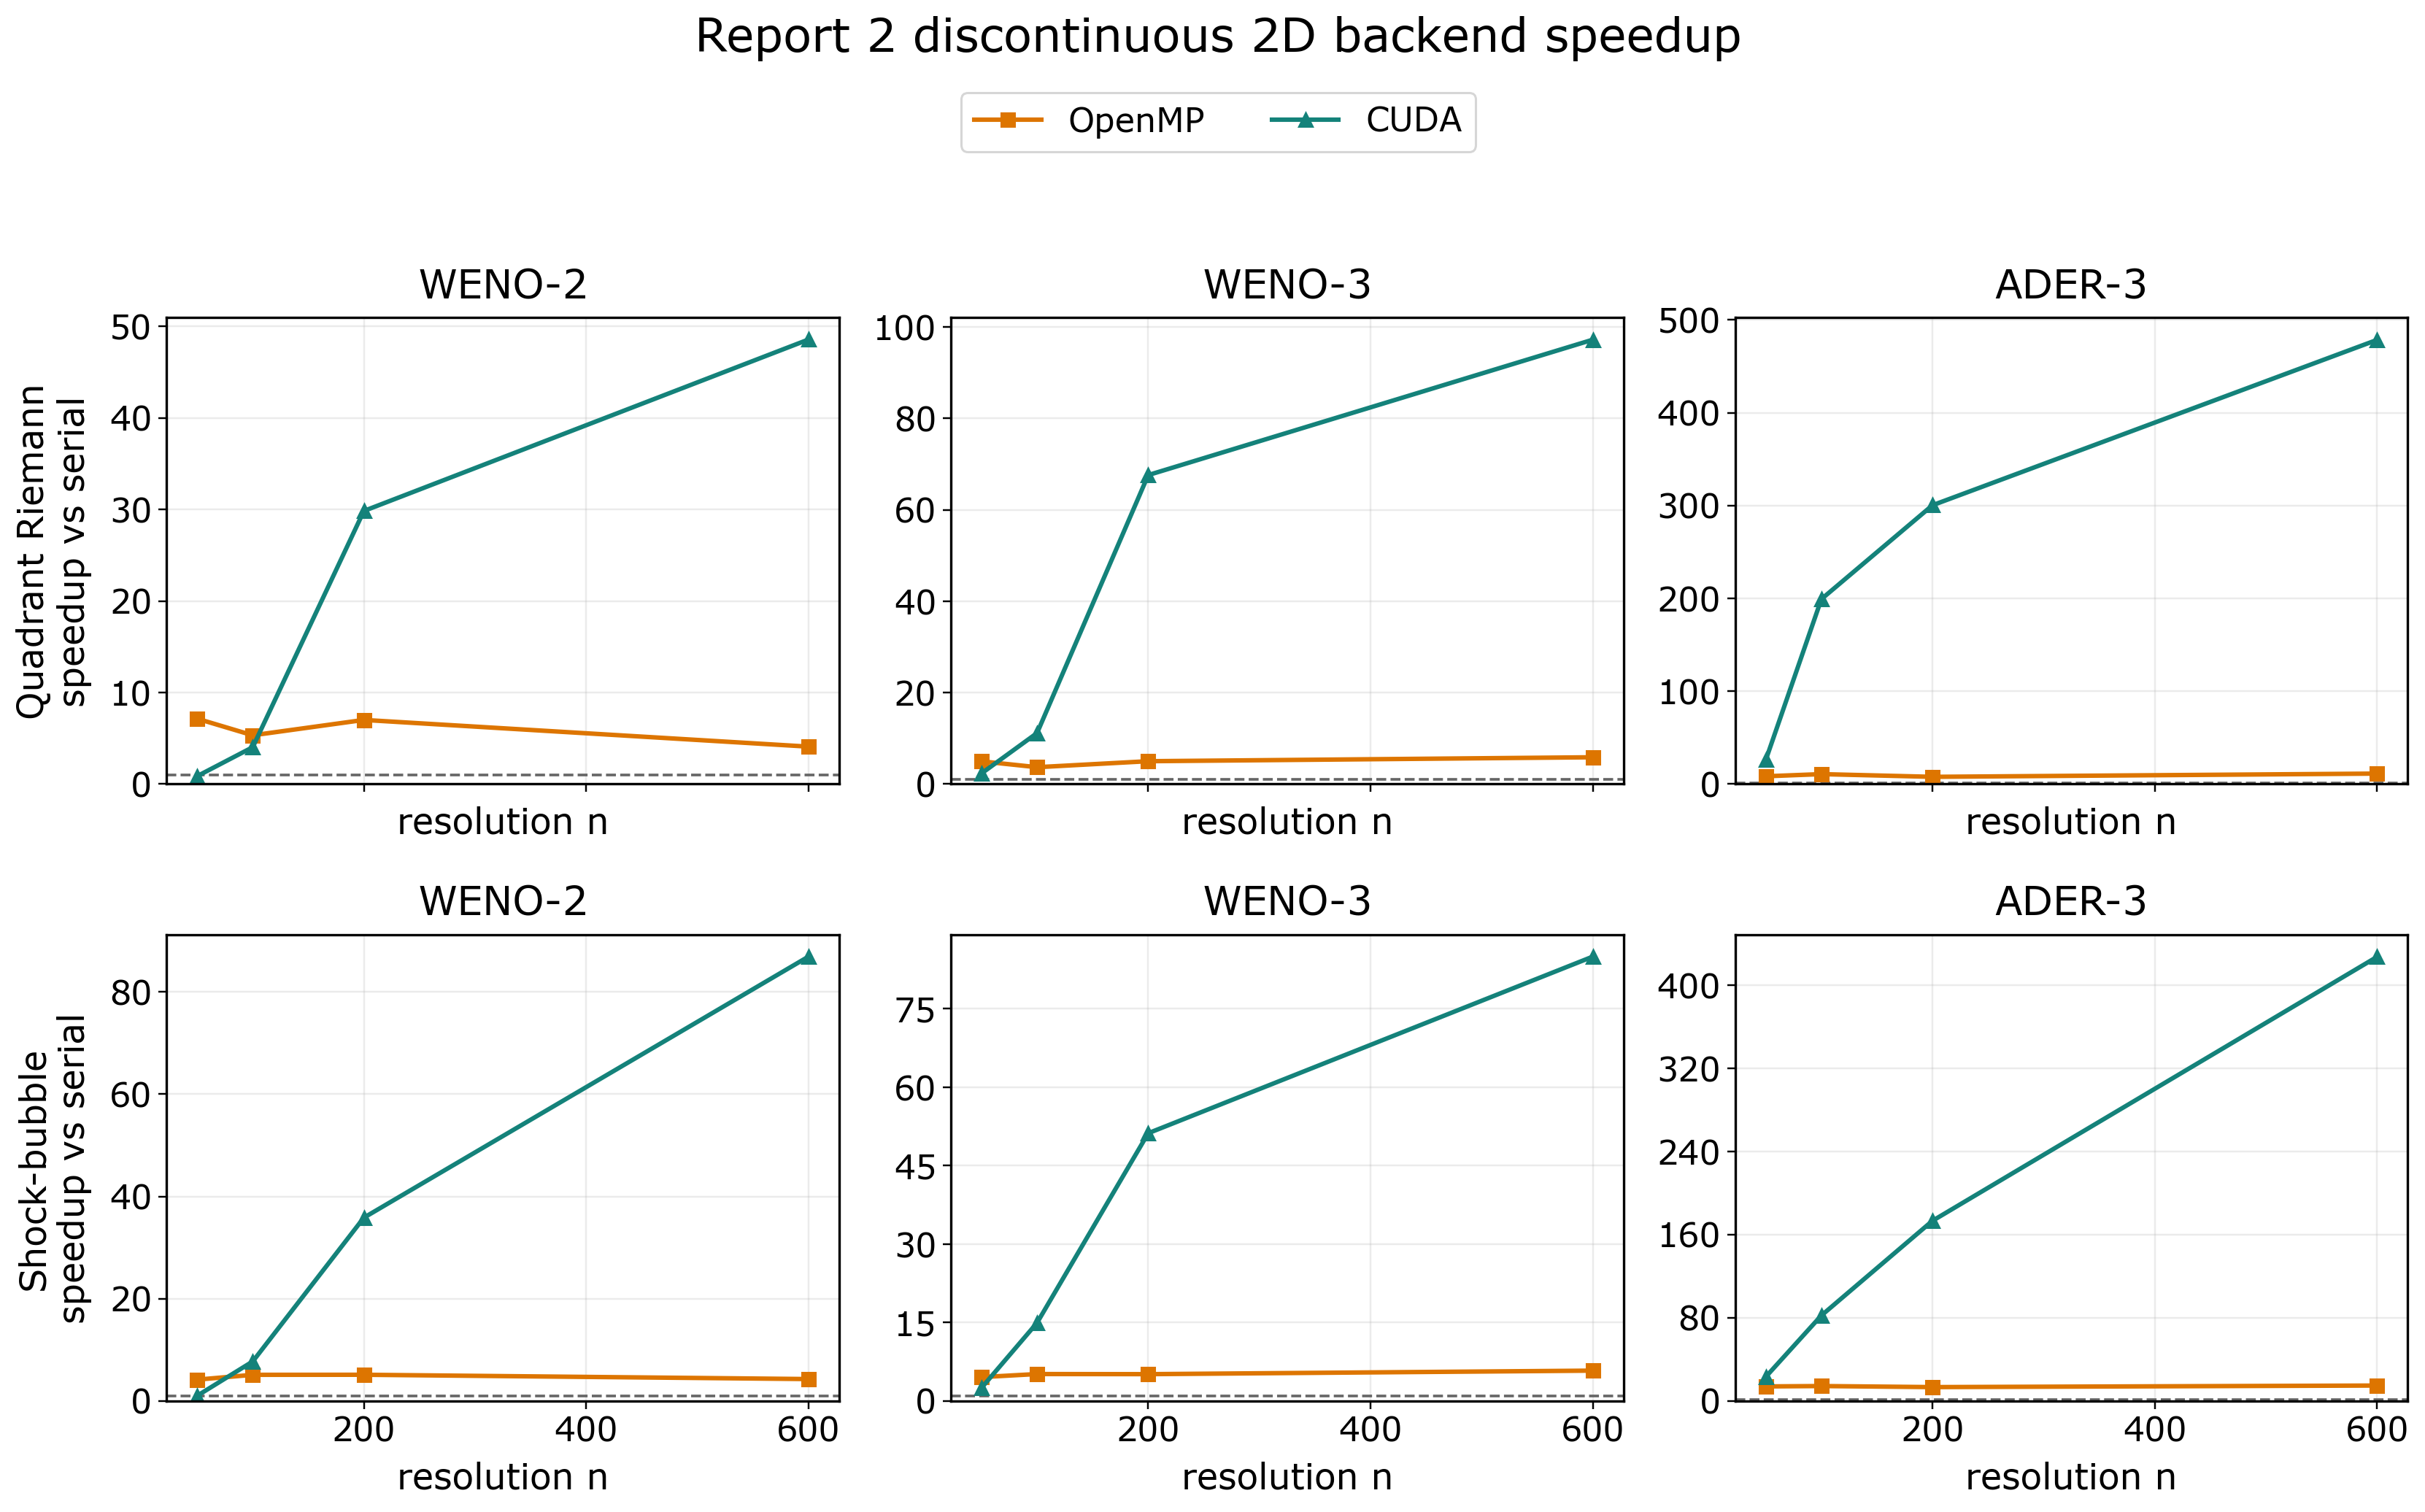
\includegraphics[width=0.94\textwidth]{performance_discontinuous_speedup_hllc.png}
\caption{OpenMP and CUDA speedup for the HLLC discontinuous campaign at
\(n=50,100,200,600\).}
\label{fig:discontinuous-speedup-performance}
\end{figure}

Figure~\ref{fig:discontinuous-speedup-performance} also exposes the crossover behaviour.
CUDA is unattractive at the smallest grids but improves rapidly once the calculation is
large enough.  OpenMP reaches its useful range earlier, then flattens because synchronization,
temporary storage, reductions, and the remaining serial work do not shrink with the same
rate as the cell-local loops.  The shock--bubble ADER-3 CUDA speedup decreases from its
\(n=200\) value to \(n=600\), but remains above 400. The result is better read as evidence
of a changing bottleneck than as a failure of acceleration.

\section{Matched HLL and HLLC comparison}

HLLC is the main Report~2 flux because it restores the contact wave omitted by HLL.  The
older HLL data are nevertheless useful in this chapter: they reveal whether the additional
wave structure changes measured accuracy and cost.  Only strict matches are used here.
The compared rows have the same problem, method, grid, CFL number, final time, backend,
and accepted time-step count, so the flux route is the intended difference.

\begin{table}[H]
\centering
\small
\begin{tabular}{lrrrrr}
\toprule
Method & HLL time & HLLC time & HLL \(L_1\) & HLLC \(L_1\) & Error change \\
\midrule
WENO-2 & 8.51 & 2.08 & \(4.746\times10^{-7}\) & \(4.703\times10^{-7}\) & \(-0.9\%\) \\
WENO-3 & 6.18 & 2.71 & \(5.112\times10^{-8}\) & \(1.726\times10^{-8}\) & \(-66.2\%\) \\
ADER-3 & 10.03 & 10.51 & \(5.063\times10^{-8}\) & \(1.681\times10^{-8}\) & \(-66.8\%\) \\
\bottomrule
\end{tabular}
\caption{Matched smooth CUDA comparison at \(600\times600\).  A negative error change
means that HLLC is more accurate.}
\label{tab:hll-hllc-n600}
\end{table}

\begin{figure}[H]
\centering
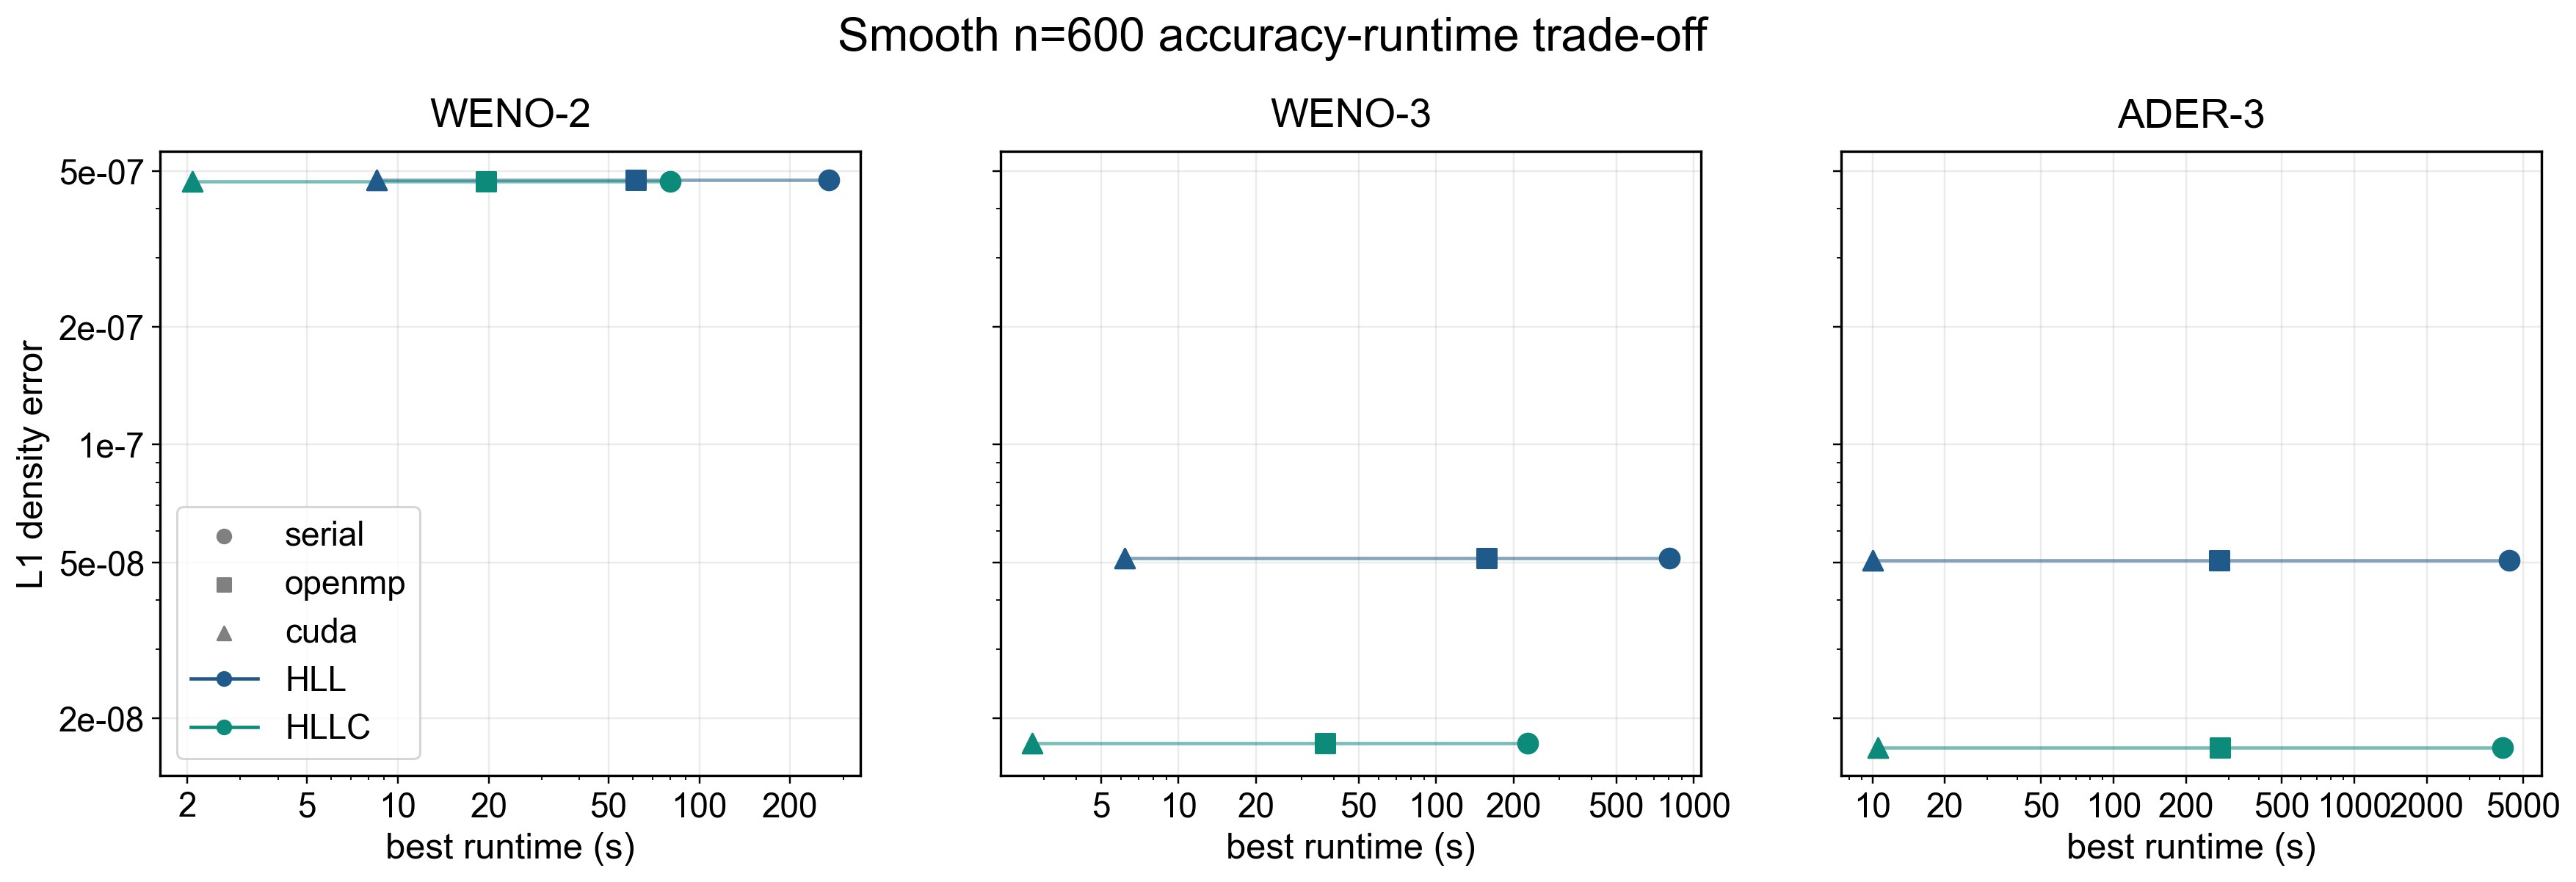
\includegraphics[width=0.96\textwidth]{performance_hll_hllc_n600_tradeoff.png}
\caption{Matched HLL--HLLC accuracy--runtime comparison at \(600\times600\).  Marker
shape identifies backend and colour identifies flux route.}
\label{fig:hll-hllc-n600-tradeoff}
\end{figure}

The flux change has little effect on WENO-2 error, but it lowers WENO-3 and ADER-3 error by
about two thirds.  This supports the physical motivation for HLLC: preserving the contact
wave matters more once the surrounding reconstruction is sufficiently accurate.  Runtime
does not follow one universal ordering.  HLLC is substantially faster for the two WENO
implementations in the stored smooth campaign, whereas ADER-3 is 4.8\% slower on CUDA.
The WENO timing gain should not be interpreted as a theorem that HLLC is intrinsically
cheaper than HLL.  It is an observed property of these complete code paths, including their
branching, memory traffic, compiler output, and accepted implementation history.

\begin{figure}[H]
\centering
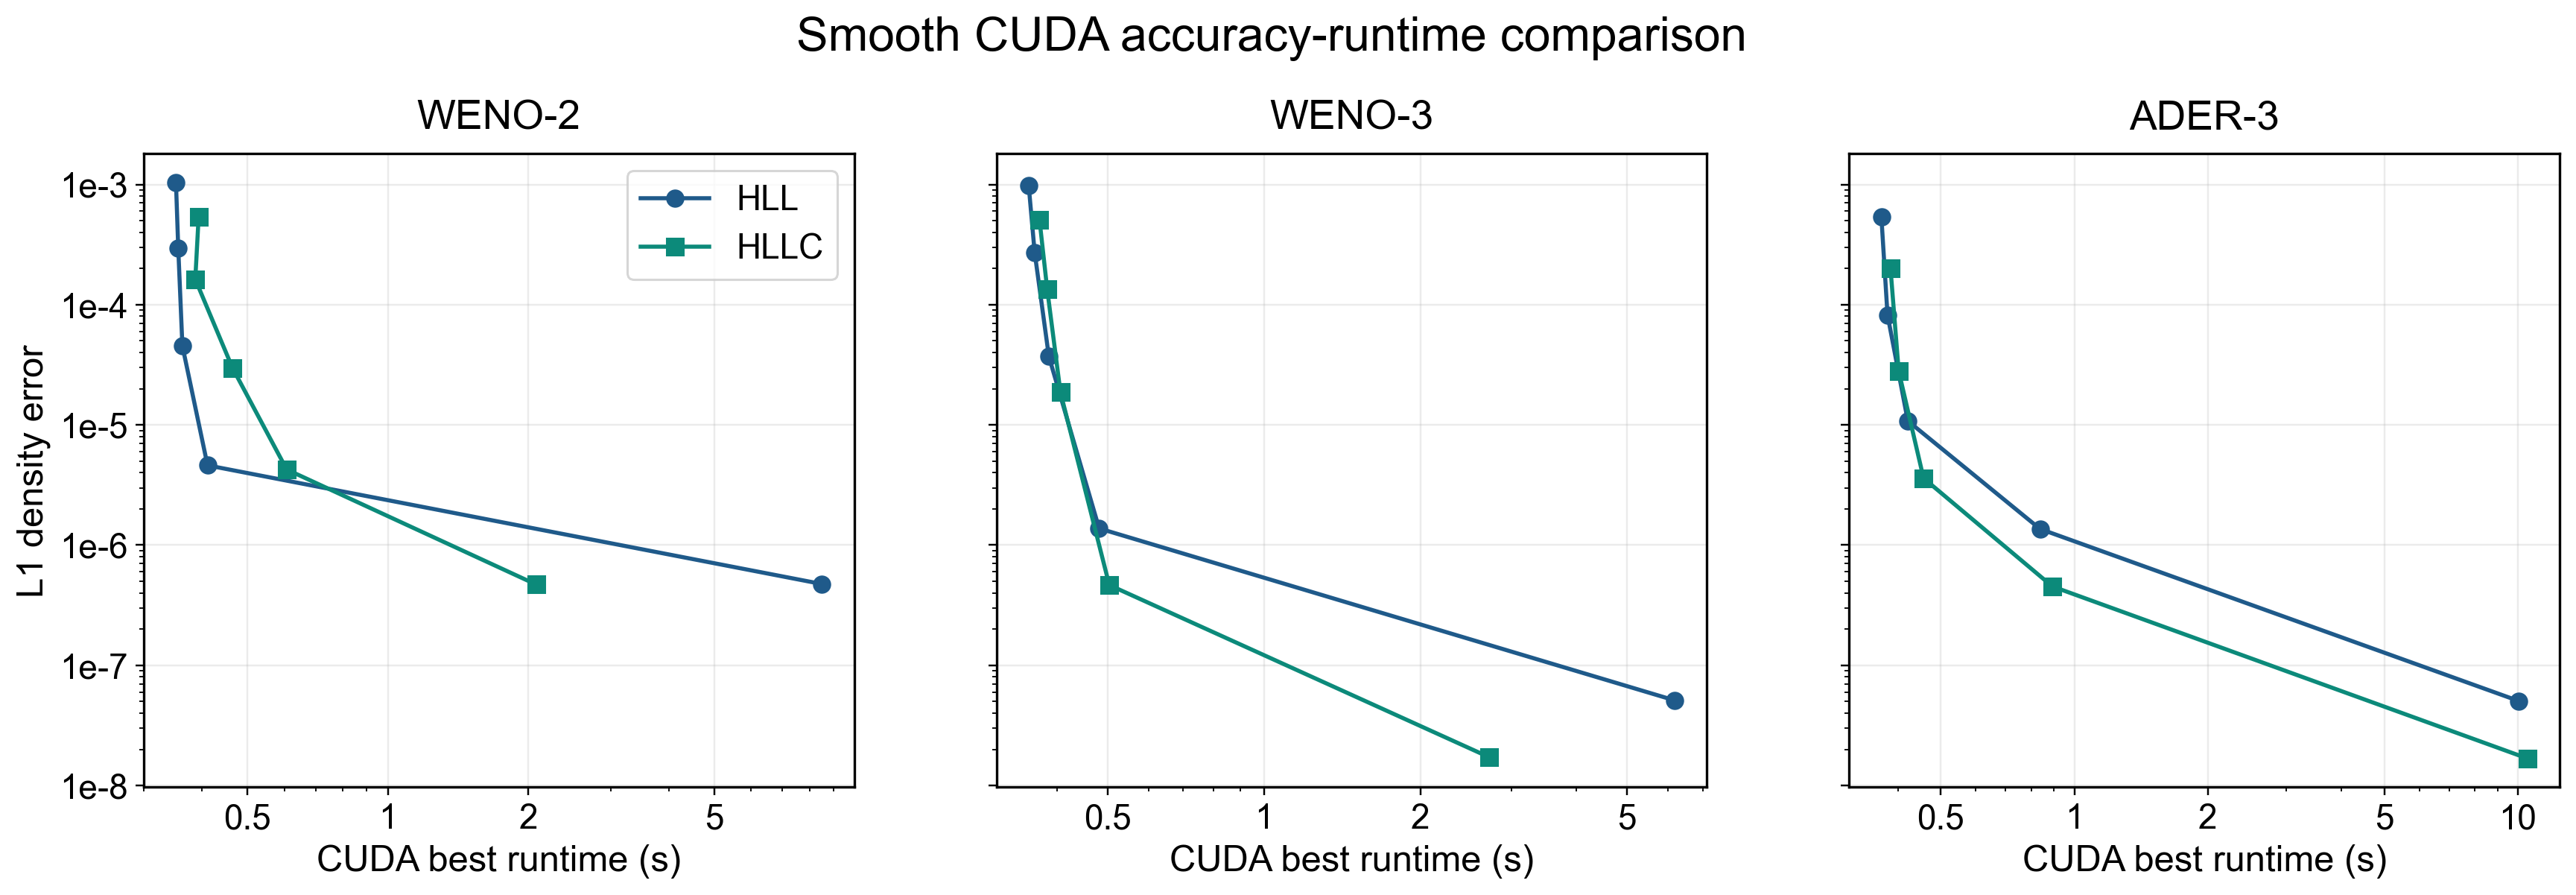
\includegraphics[width=0.92\textwidth]{performance_hll_hllc_cuda_tradeoff.png}
\caption{Matched smooth CUDA accuracy--runtime trajectories for HLL and HLLC across the
common grid sequence.}
\label{fig:hll-hllc-cuda-tradeoff}
\end{figure}

Figure~\ref{fig:hll-hllc-cuda-tradeoff} confirms that the \(600^2\) result is not an
isolated endpoint.  For WENO-3 and ADER-3, the HLLC curve remains below the HLL curve over
the refinement sequence, so it reaches a lower density error for a comparable cost.  The
HLL evidence therefore strengthens rather than displaces the HLLC conclusion: HLLC is the
appropriate authoritative dataset, while HLL provides a useful performance baseline.

\section{Phase-resolved acceleration and bottlenecks}

End-to-end speedup identifies the best backend but does not explain why it wins.  A separate
instrumented campaign therefore accumulated time in five groups:
\begin{itemize}[leftmargin=1.8em]
  \item setup/workspace/transfer: initialization, temporary flux arrays, and explicit
        host--device transfer timing.
  \item CFL reduction: characteristic-speed evaluation and the global maximum reduction.
  \item spatial operator: reconstruction or local prediction, HLLC interface fluxes, and
        assembly of the spatial residual.
  \item update/validity: conservative state update, admissibility checks, and retry logic.
  \item other: profiled time not assigned to the preceding categories.
\end{itemize}
The profiler was run at \(100^2\), where fixed costs are visible, and \(600^2\), where
the stencil work dominates.  Three repeats were used at \(100^2\). The \(600^2\) profiles
are single diagnostic runs.

\begin{figure}[H]
\centering
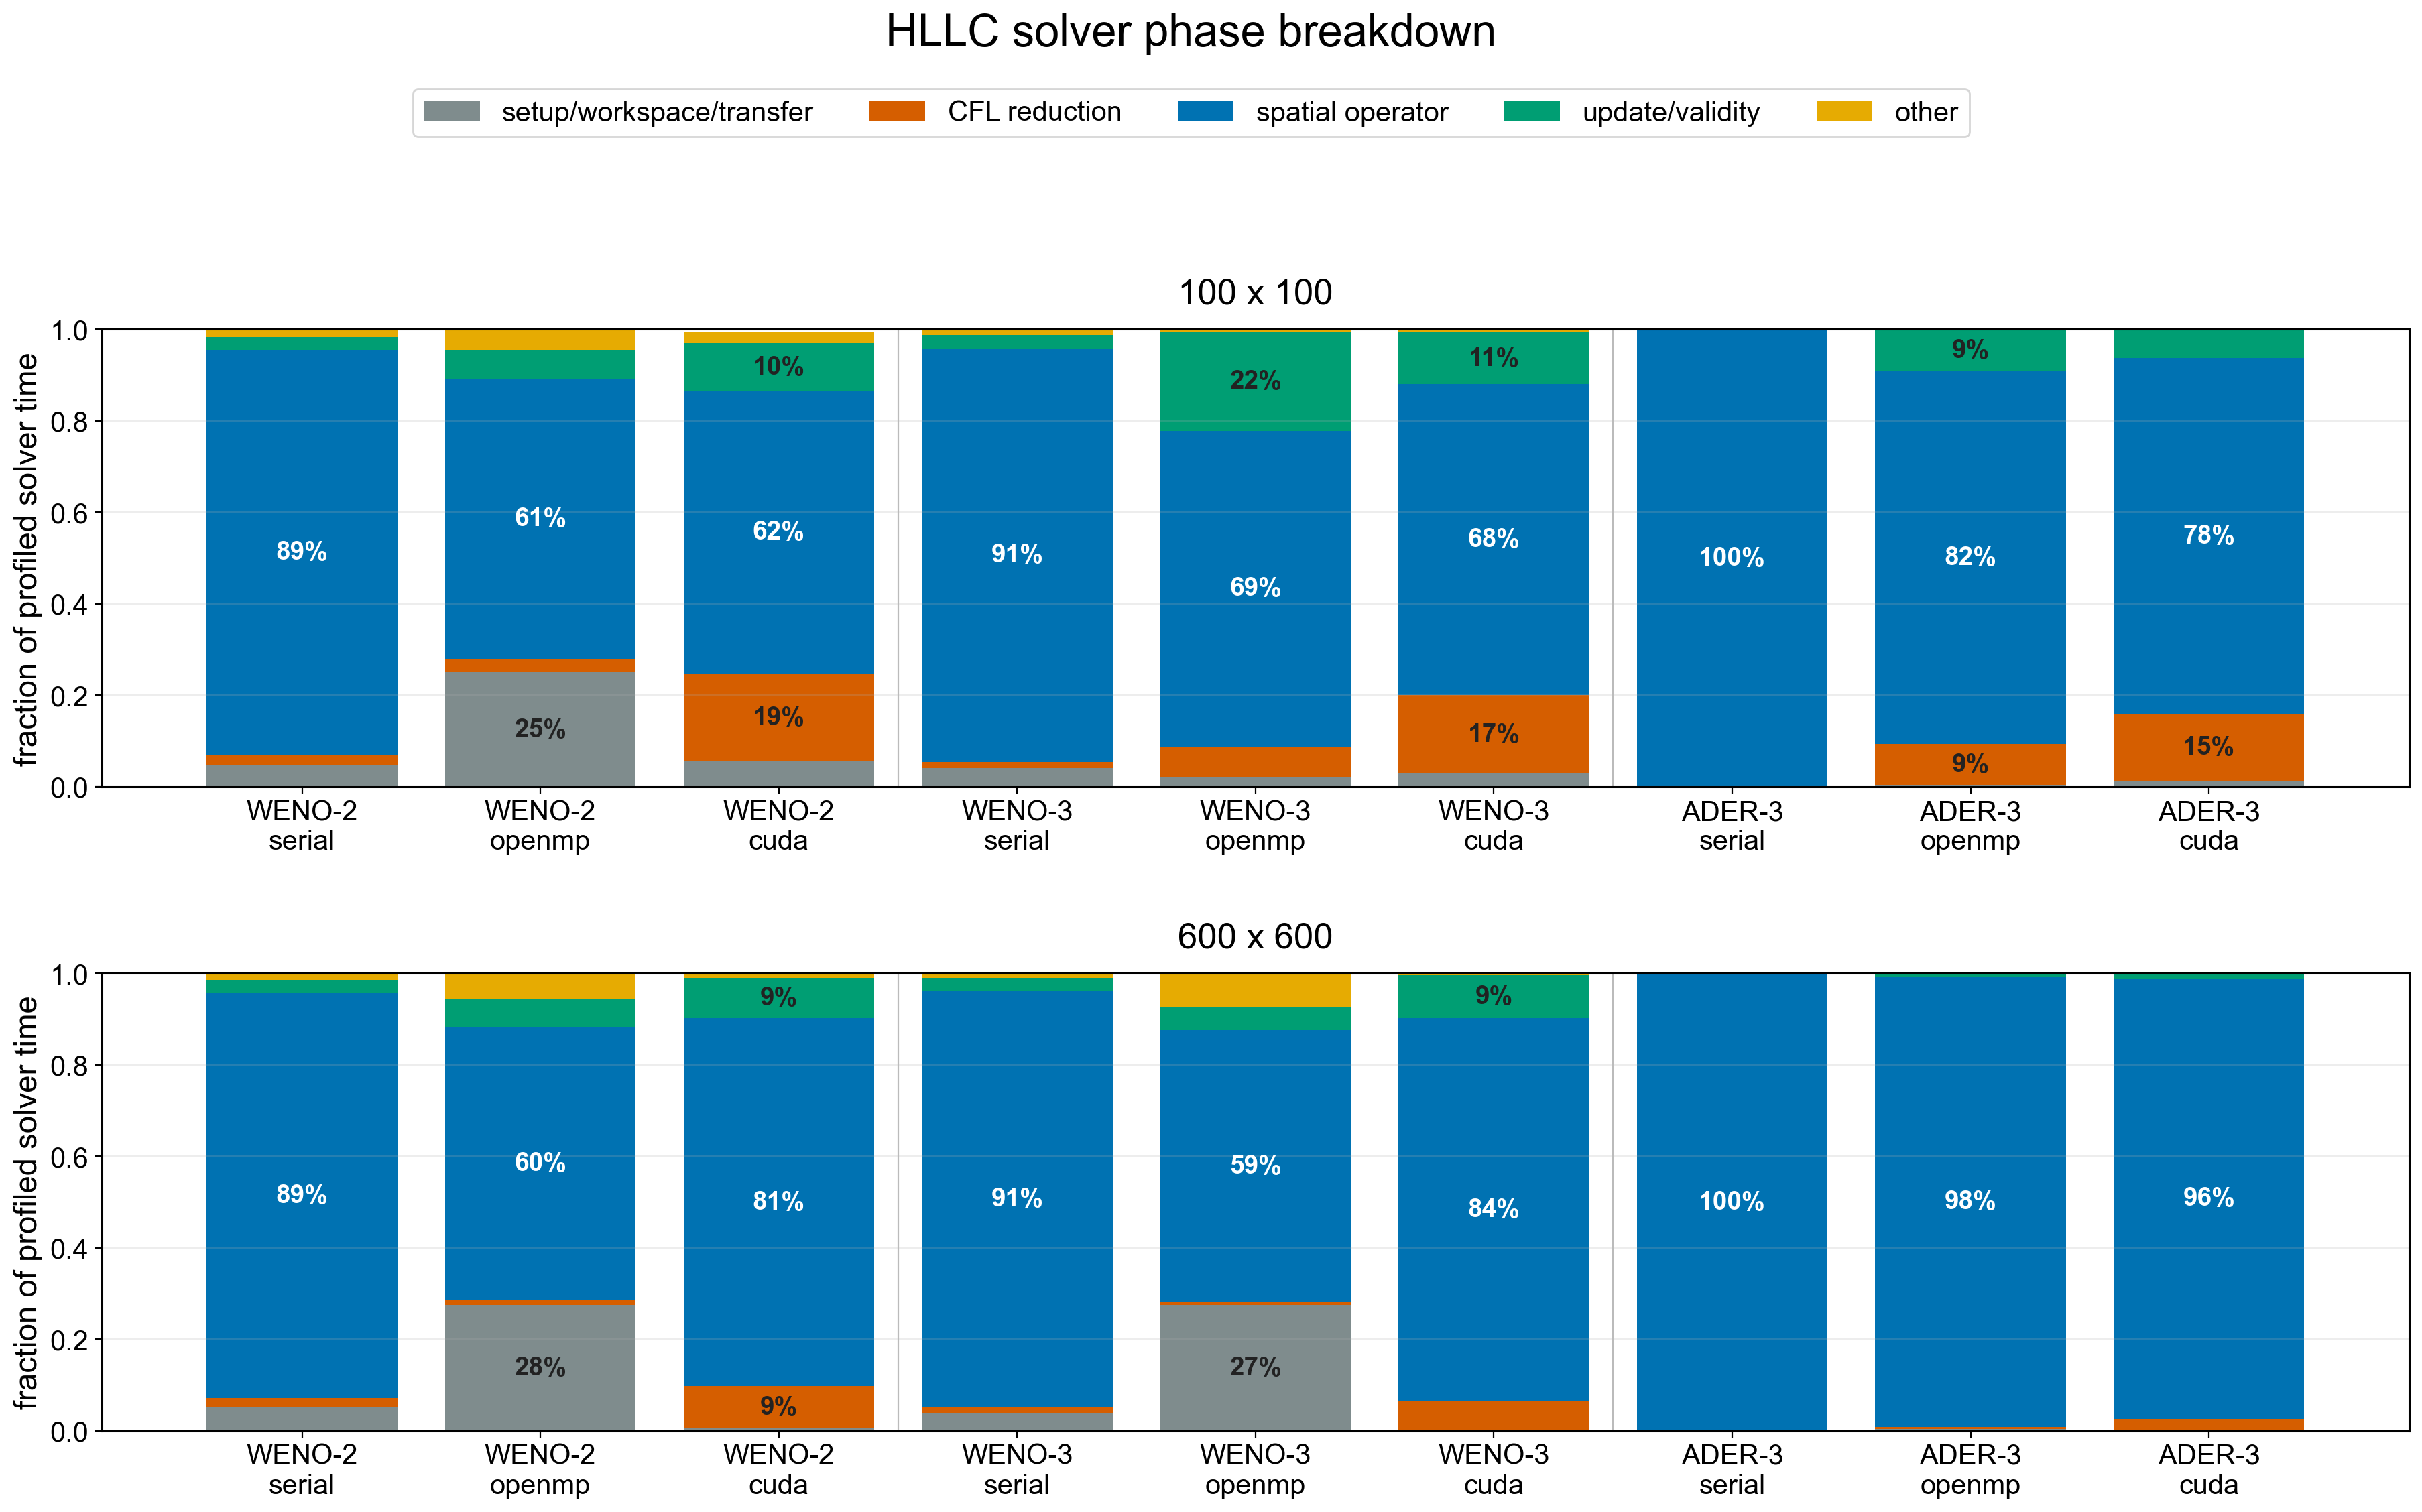
\includegraphics[width=0.98\textwidth]{performance_phase_breakdown_hllc.png}
\caption{Fraction of instrumented HLLC solver time assigned to each phase at
\(100\times100\) and \(600\times600\).}
\label{fig:phase-breakdown-performance}
\end{figure}

The spatial operator is the principal cost in every large-grid run.  Its serial share is
88.6\% for WENO-2, 91.0\% for WENO-3, and 99.7\% for ADER-3.  On OpenMP, the WENO share
falls to about 59.5\% because workspace management and the less scalable update phases
become visible after the main loops are accelerated.  ADER-3 remains 98.4\% spatial on
OpenMP because its local predictor is so expensive that fixed overhead is comparatively
small.  On CUDA, the spatial shares are 80.5\%, 83.8\%, and 96.3\%. The residual CFL and
state-update phases account for most of the remaining time.

\begin{table}[H]
\centering
\small
\begin{tabular}{lrrr|rr}
\toprule
& \multicolumn{3}{c|}{Spatial share (\%)} & \multicolumn{2}{c}{Spatial speedup} \\
Method & Serial & OpenMP & CUDA & OpenMP & CUDA \\
\midrule
WENO-2 & 88.6 & 59.5 & 80.5 & 12.20 & 204.06 \\
WENO-3 & 91.0 & 59.5 & 83.8 & 10.52 & 205.64 \\
ADER-3 & 99.7 & 98.4 & 96.3 & 11.36 & 1049.00 \\
\bottomrule
\end{tabular}
\caption{Spatial-operator share and comparable phase speedup at \(600\times600\).
Phase speedups are relative to the instrumented serial phase for the same method.}
\label{tab:phase-spatial}
\end{table}

\begin{figure}[H]
\centering
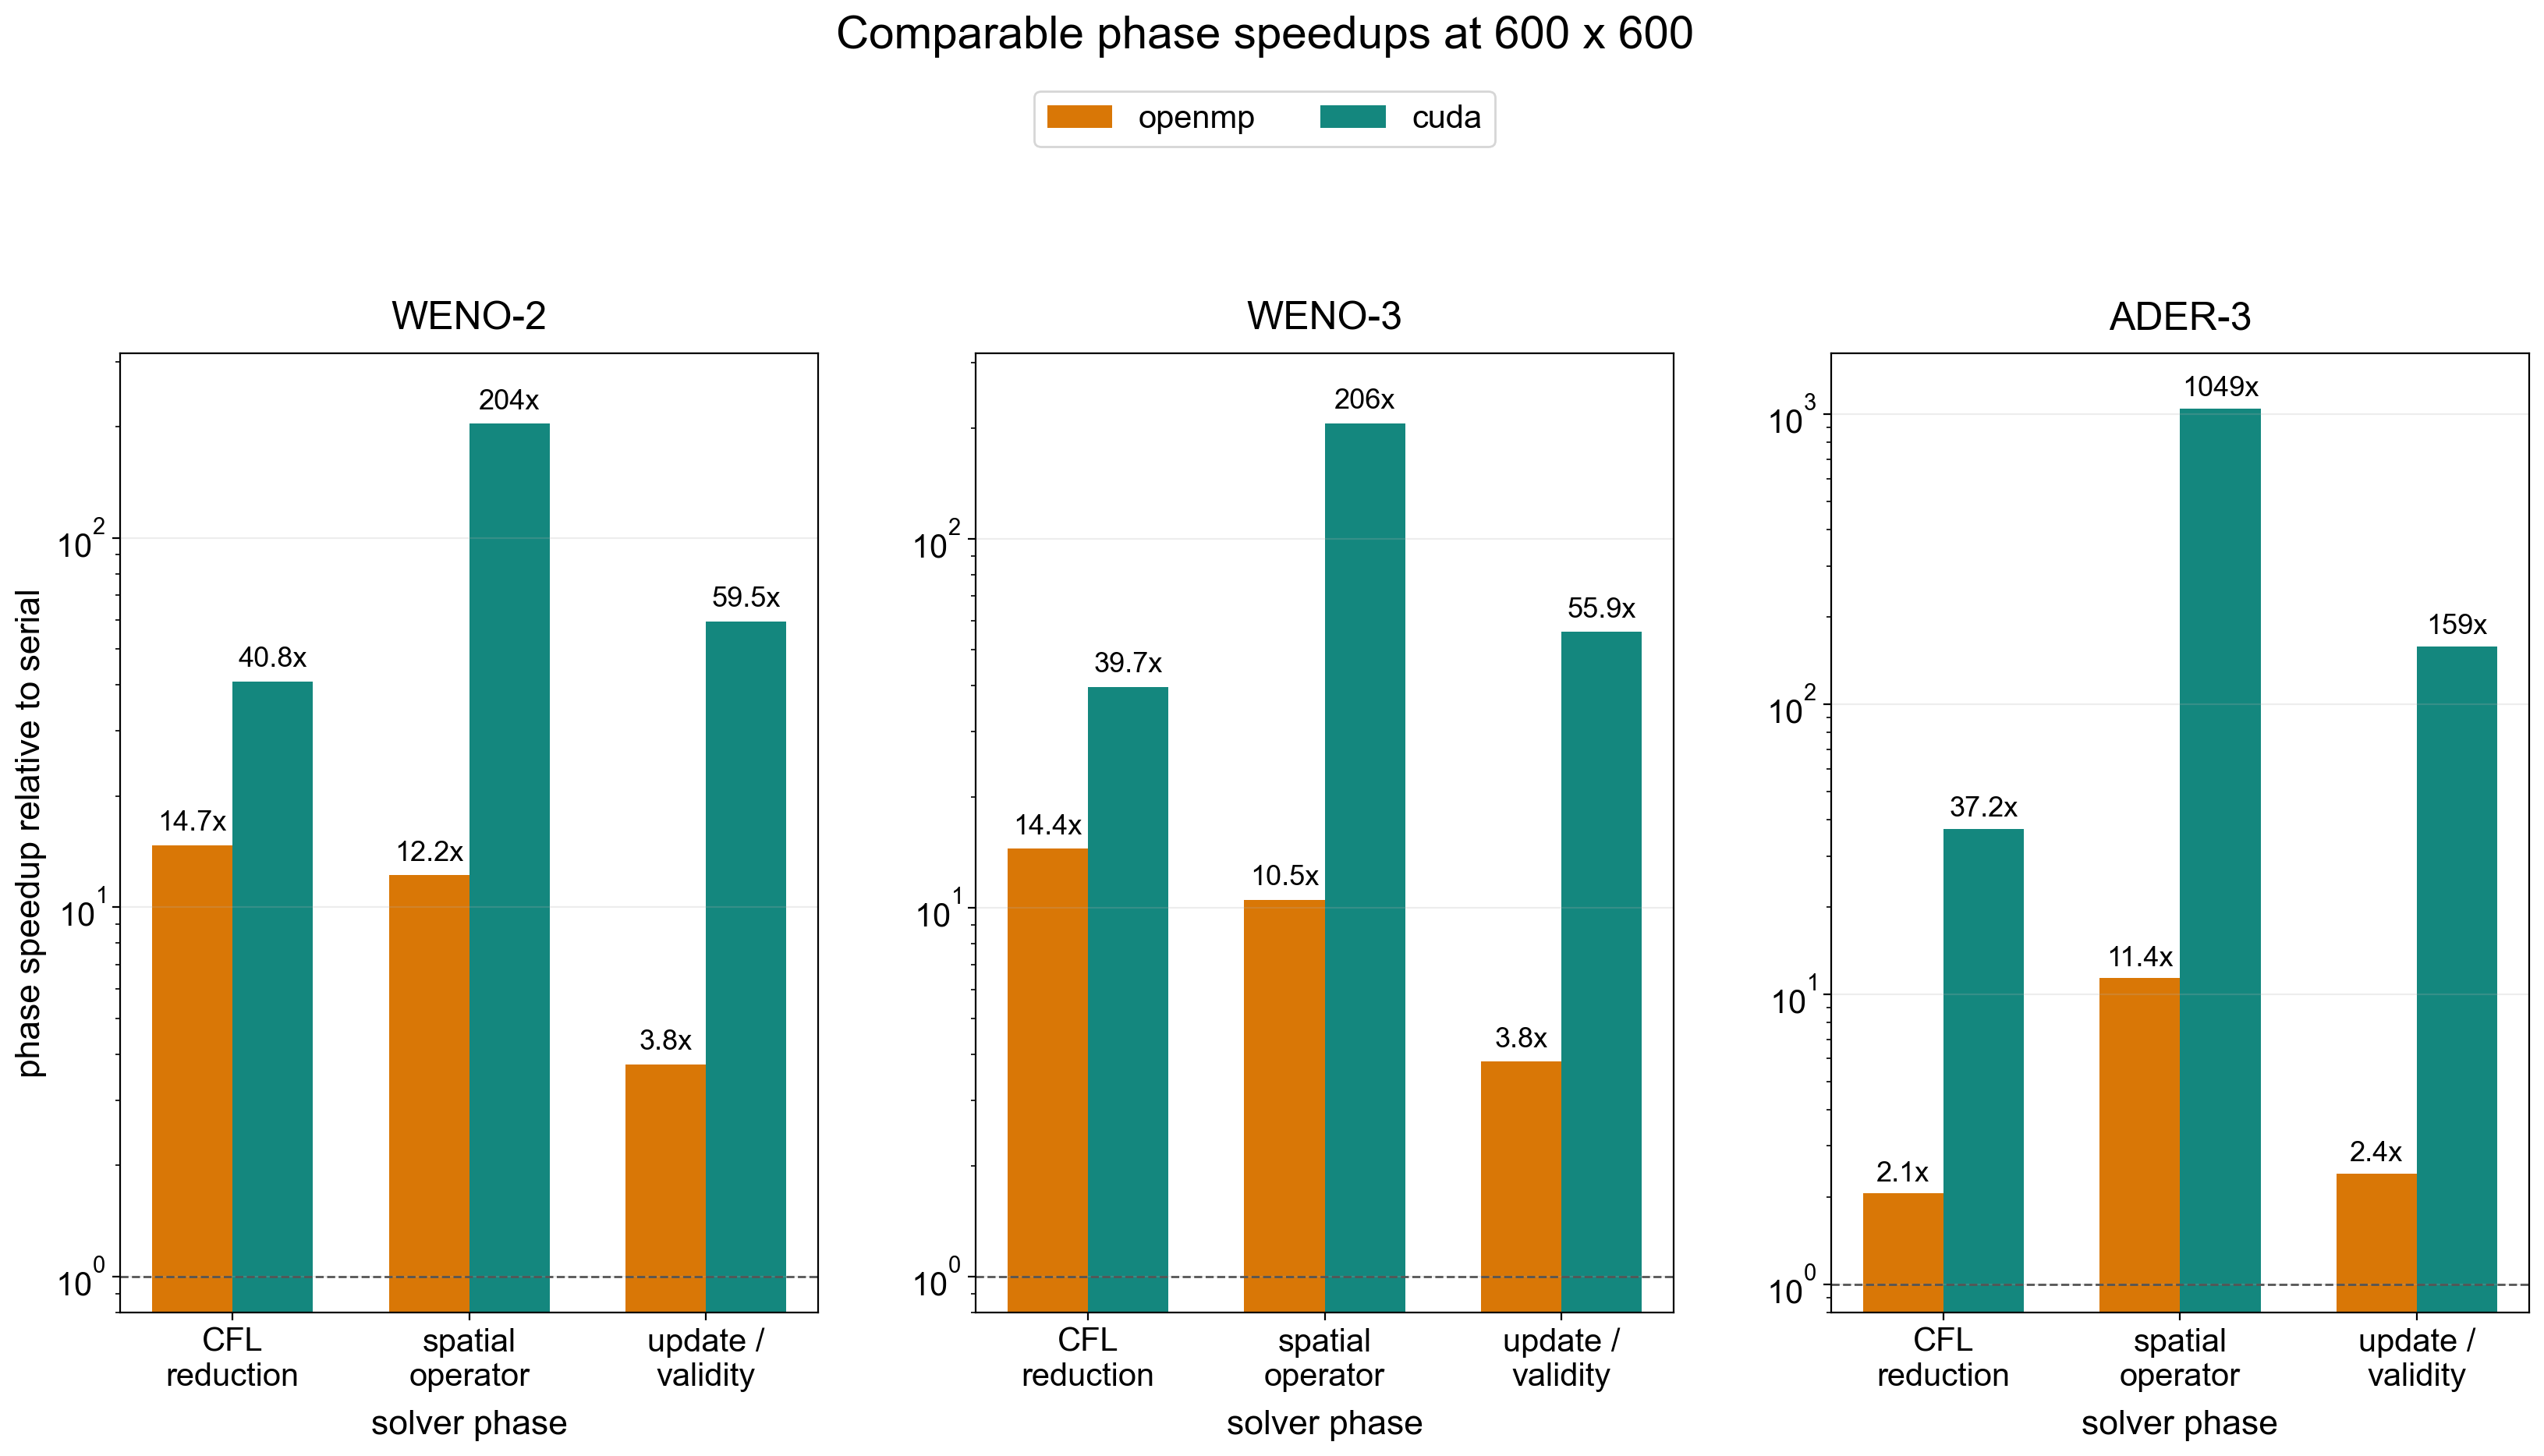
\includegraphics[width=0.98\textwidth]{performance_phase_speedup_hllc.png}
\caption{Comparable HLLC phase speedups at \(600\times600\).  The aggregate
setup/workspace/transfer category is omitted because its CPU and CUDA implementation
boundaries are not identical.}
\label{fig:phase-speedup-performance}
\end{figure}

Figure~\ref{fig:phase-speedup-performance} gives the clearest optimization priorities.
CUDA reduces the WENO spatial operators by about 204--206 times and the ADER-3 spatial
operator by roughly 1049 times.  Once that dominant work is accelerated, CFL reduction and
the final update become the limiting fractions. This is the expected Amdahl-type shift
\cite{amdahl1967}.
For OpenMP, the spatial loops still accelerate by approximately 10.5--12.2 times, but
end-to-end WENO speedup is reduced by workspace allocation, synchronization, and update
work.  ADER-3 has an additional OpenMP bottleneck: its CFL and update phases accelerate by
only about 2.05 and 2.41, respectively, even though the predictor-dominated spatial phase
scales well.

The phase measurements are diagnostic, not replacements for the canonical timings in
Table~\ref{tab:smooth-n600-performance}.  CUDA phase boundaries require explicit
synchronization to obtain meaningful kernel times, and those synchronizations change the
measured total.  The profiler is therefore used to assign cost and identify bottlenecks.
All headline runtime and speedup claims continue to use the ordinary no-output campaign.

\section{OpenMP thread scaling}

The thread experiment isolates CPU scaling on the smooth \(100^2\) case using the OpenMP
shared-memory model \cite{openmp52} and \(p=1,2,4,8,16\).
Table~\ref{tab:openmp-thread-scaling} and
Figure~\ref{fig:openmp-thread-scaling-performance} show that method complexity determines
how long additional threads remain useful.  WENO-2 reaches only 4.20 times speedup at 16
threads, equivalent to 26.3\% parallel efficiency. WENO-3 reaches 5.33 and 33.3\%.
ADER-3 reaches 14.30 and 89.4\%, because its compute-heavy predictor supplies enough
independent work to dominate thread launch, synchronization, and memory-management costs.
The bounded efficiencies are consistent with Amdahl's observation that non-parallel work
limits total speedup even when the dominant loop scales well \cite{amdahl1967}.

\begin{table}[H]
\centering
\begin{tabular}{lrrrr}
\toprule
Method & \(T_1\) (s) & \(T_{16}\) (s) & \(S_{16}\) & \(E_{16}\) \\
\midrule
WENO-2 & 0.4483 & 0.1066 & 4.20 & 26.3\% \\
WENO-3 & 1.0475 & 0.1966 & 5.33 & 33.3\% \\
ADER-3 & 19.1913 & 1.3422 & 14.30 & 89.4\% \\
\bottomrule
\end{tabular}
\caption{HLLC OpenMP scaling from one to 16 threads at \(100\times100\).}
\label{tab:openmp-thread-scaling}
\end{table}

\begin{figure}[H]
\centering
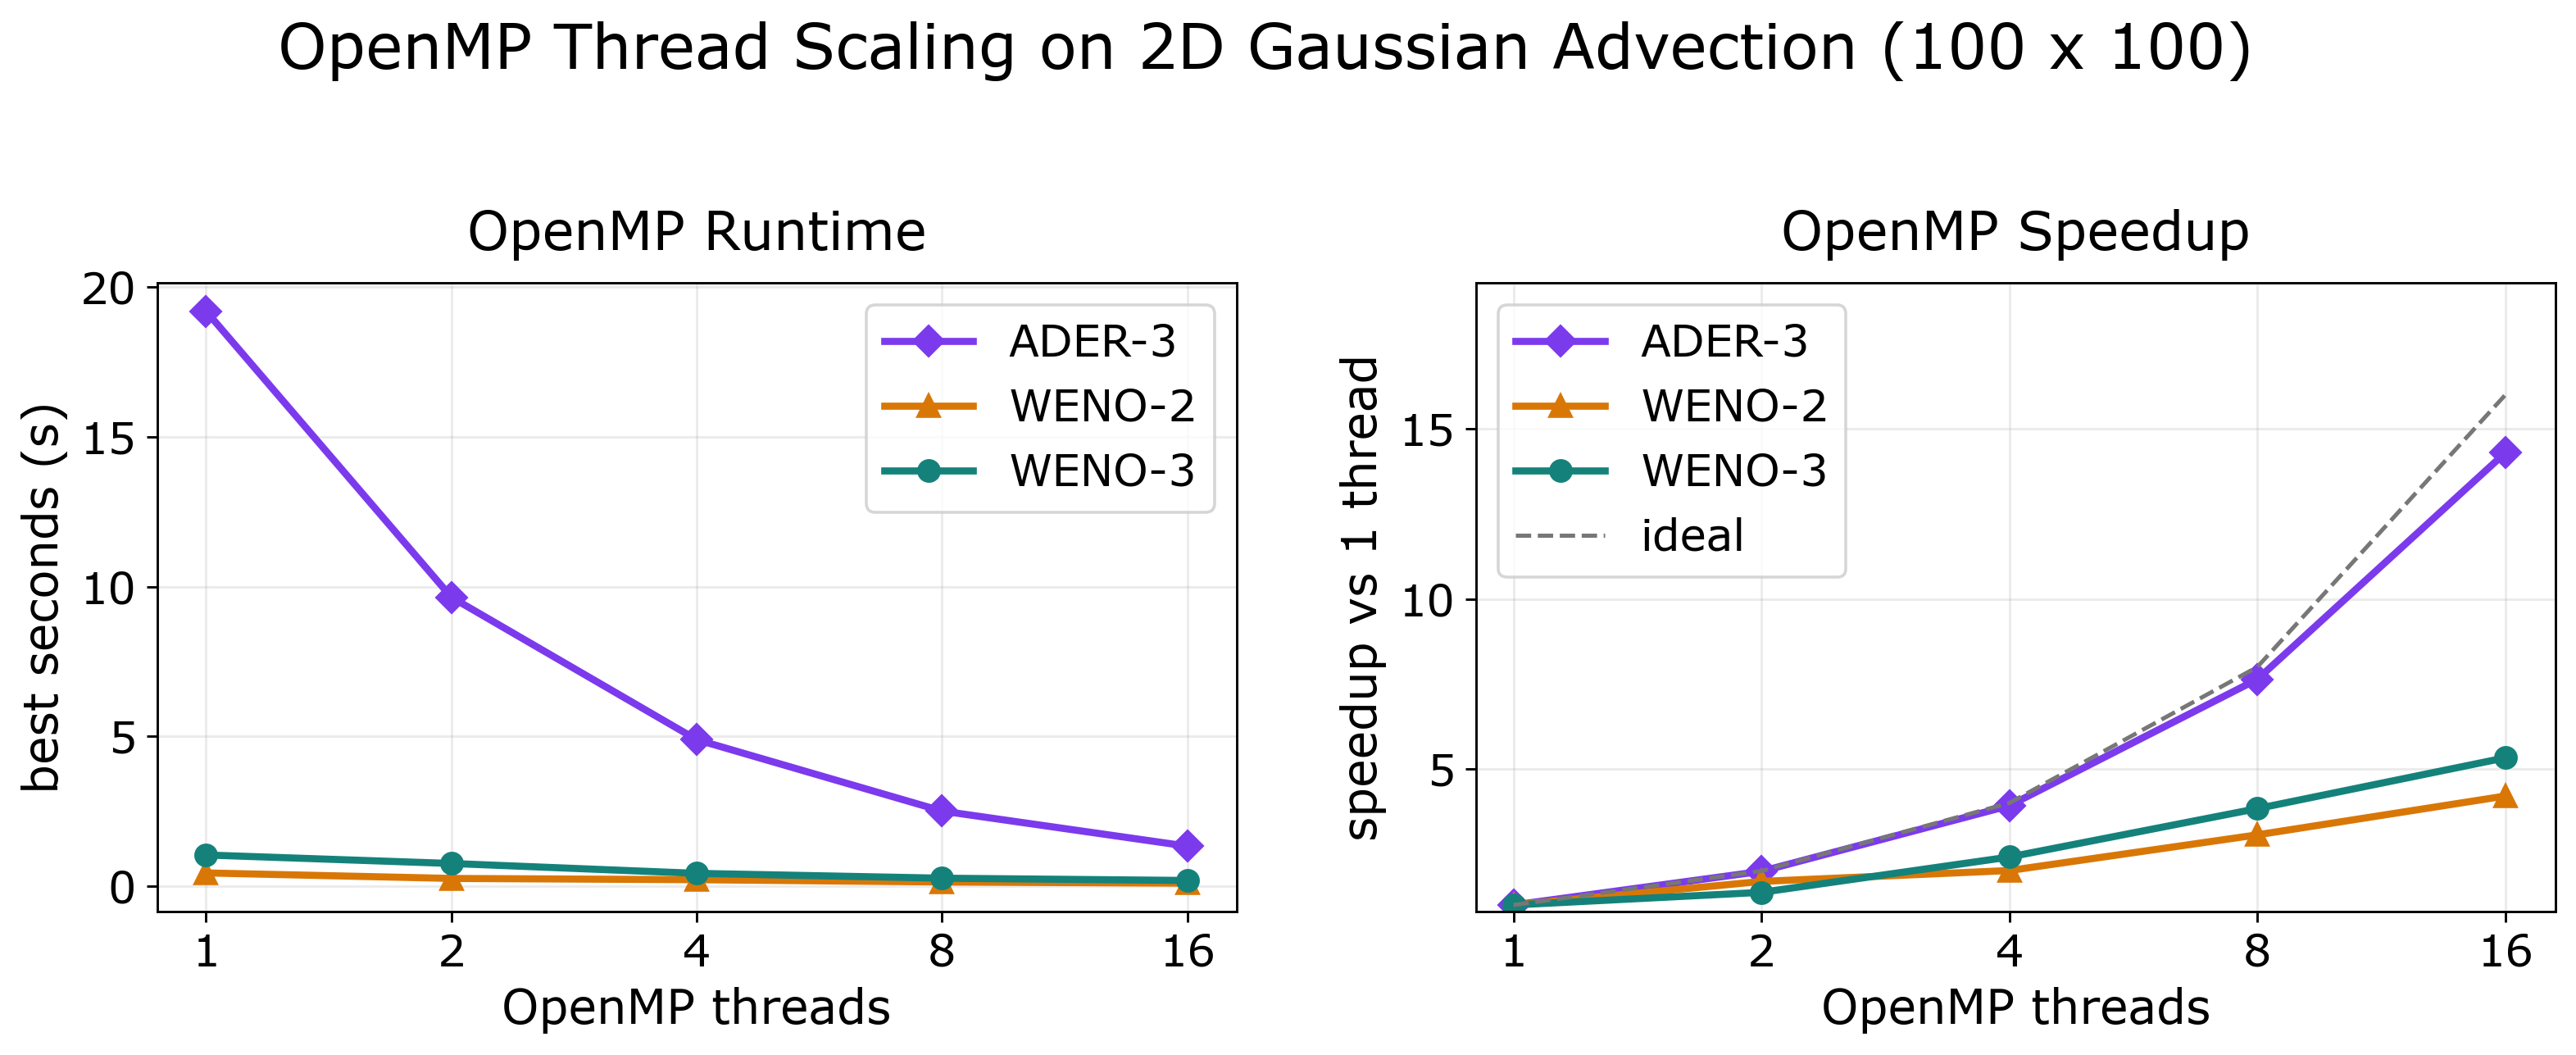
\includegraphics[width=0.88\textwidth]{performance_openmp_threads_hllc.png}
\caption{HLLC OpenMP runtime and speedup at \(100\times100\).  The corresponding
16-thread parallel efficiencies are listed in Table~\ref{tab:openmp-thread-scaling}.}
\label{fig:openmp-thread-scaling-performance}
\end{figure}

The early saturation of WENO-2 is therefore not evidence that its numerical method has
failed. It is a workload-granularity result.  A cheaper stencil leaves a larger fraction of
the run in work that is fixed, memory-bound, or repeatedly synchronized.  ADER-3 is the
opposite case: it is expensive in absolute terms, but that expense is highly parallel.

\section{CUDA scaling envelope}

The all-backend campaign stops at \(600^2\) because serial ADER-3 is already very slow.
A CUDA-only sweep extends the smooth calculation to ten resolutions between \(n=600\)
and \(n=5000\).  The sampled sequence is
\(600, 1000, 1400, 1800, 2400\), followed by
\(3000, 3600, 4200, 4600,\) and \(5000\).  In a two-dimensional explicit scheme the
number of cells scales as \(n^2\), while the CFL condition makes the number of time steps
approximately proportional to \(n\).  A well-behaved large-grid runtime is therefore
expected to approach
\begin{equation}
  T(n)\propto n^3.
  \label{eq:cubic-work}
\end{equation}
Here \(n\) is the number of cells in each coordinate direction and \(T(n)\) is
the measured CUDA runtime on the resulting \(n\times n\) grid.
The local empirical exponent between adjacent points is
\begin{equation}
  p_{12}=\frac{\log(T_2/T_1)}{\log(n_2/n_1)}.
  \label{eq:local-runtime-exponent}
\end{equation}
The subscripts 1 and 2 identify two consecutive grid sizes:
\(T_1=T(n_1)\) and \(T_2=T(n_2)\). Therefore \(p_{12}\approx3\) is consistent
with the expected cubic work growth, while a substantially larger value marks
a locally steeper runtime increase. It is a scaling diagnostic, not a formal
accuracy order.

\begin{figure}[H]
\centering
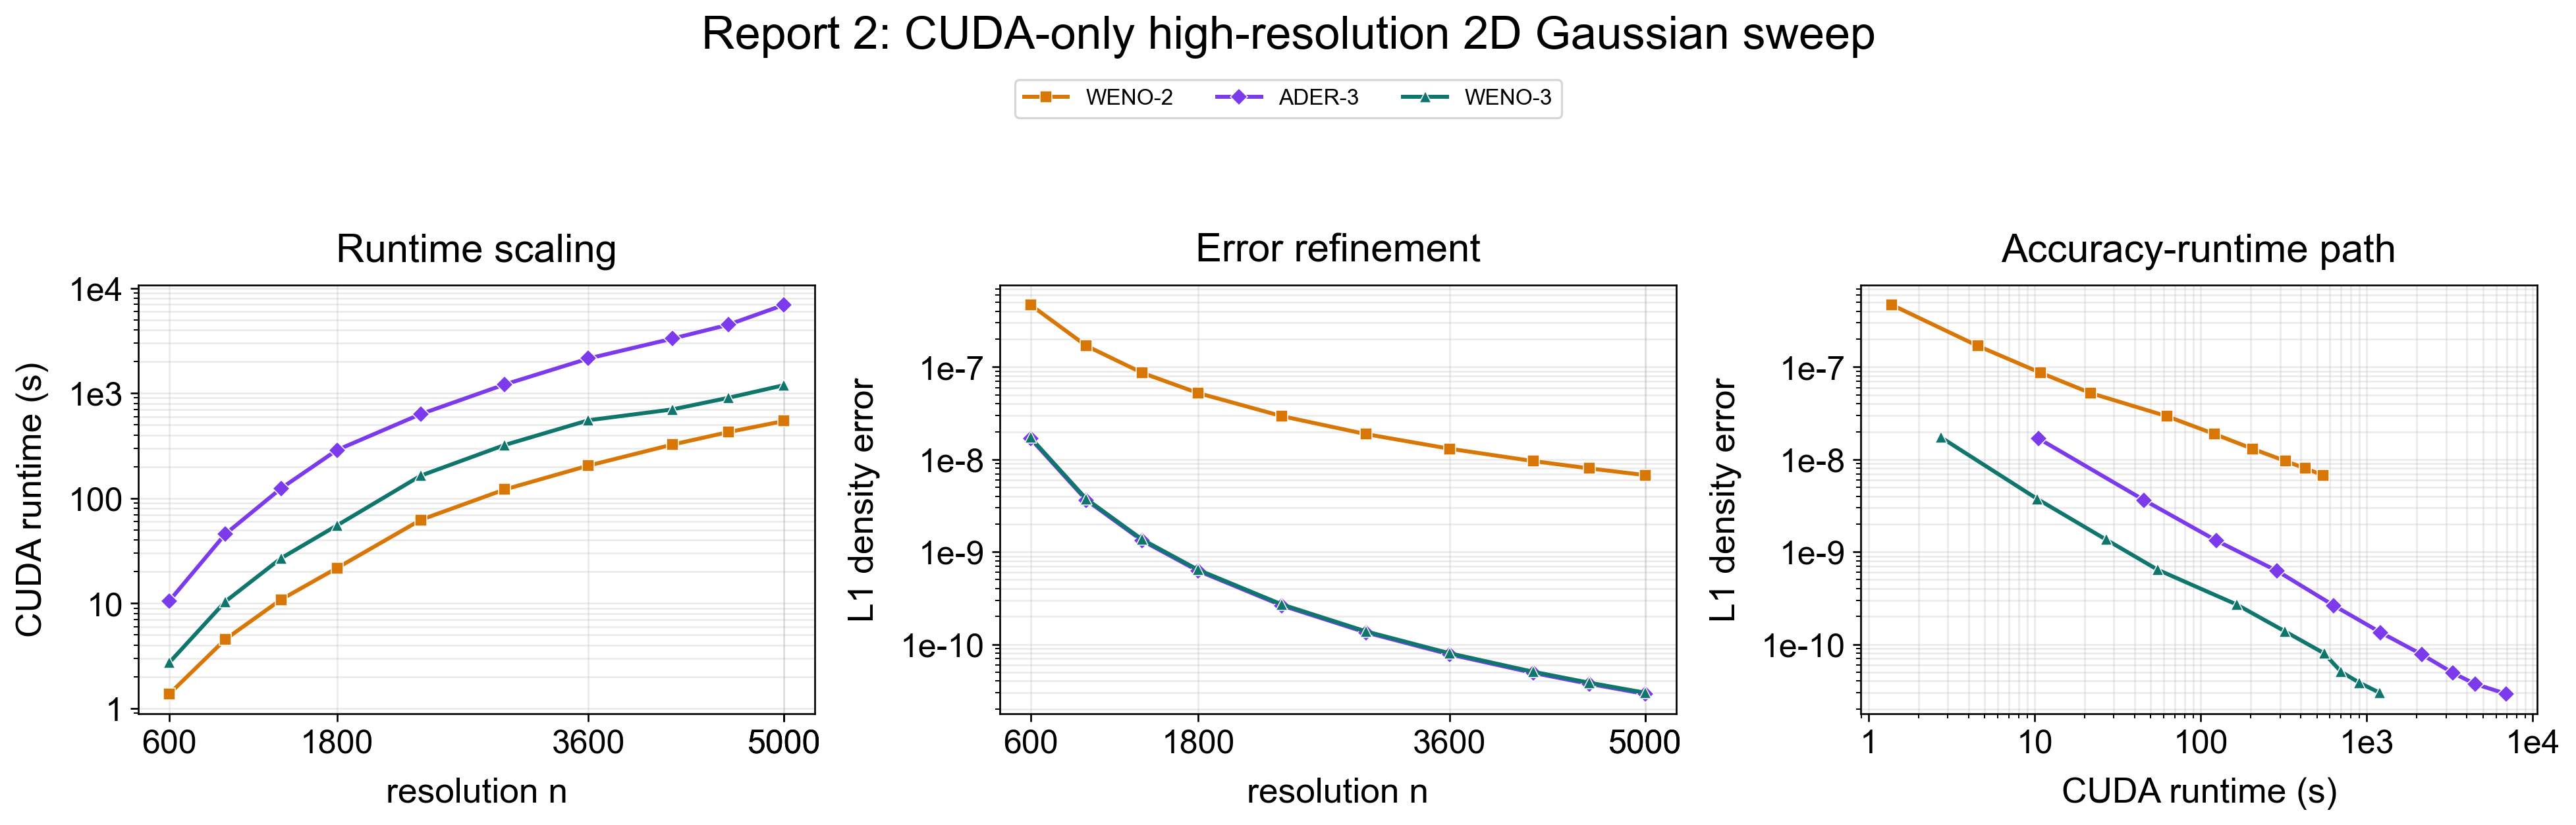
\includegraphics[width=0.98\textwidth]{performance_gpu_limit_hllc.png}
\caption{HLLC CUDA-only large-grid runtime, density error, and accuracy--runtime
trade-off through the official \(5000\times5000\) endpoint.}
\label{fig:gpu-envelope-performance}
\end{figure}

\begin{table}[H]
\centering
\begin{tabular}{lrrr}
\toprule
Method & \(T(5000)\) (s) & \(L_1(\rho)\) & Final \(p_{12}\) \\
\midrule
WENO-2 & 543.78 & \(6.769\times10^{-9}\) & 2.92 \\
WENO-3 & 1193.21 & \(2.996\times10^{-11}\) & 3.34 \\
ADER-3 & 6935.73 & \(2.908\times10^{-11}\) & 5.24 \\
\bottomrule
\end{tabular}
\caption{Largest official HLLC CUDA point and final-interval runtime exponent.  The final
exponent is a one-repeat diagnostic and is not treated as a precise hardware limit.}
\label{tab:gpu-limit-endpoint}
\end{table}

Across the complete \(600\)--\(5000\) sweep, the resolution increases by a factor of
\(8.333\), so ideal cubic work would increase by \(8.333^3=578.7\).  The measured runtime
factors are \(395.5\), \(436.9\), and \(657.2\) for WENO-2, WENO-3, and ADER-3,
respectively.  Equation~\eqref{eq:local-runtime-exponent} applied to the two endpoints
therefore gives overall exponents of \(2.82\), \(2.87\), and \(3.06\).  WENO-2 and WENO-3
grow slightly less rapidly than the nominal work count because the larger grids amortise
fixed launch and setup costs more effectively. ADER-3 is almost exactly cubic over the
full range despite its steeper final segment.

The error reduction is equally diagnostic.  From \(600^2\) to \(5000^2\),
\(L_1(\rho)\) falls by factors of \(69.5\), \(576.1\), and \(578.2\).  These values closely
match the theoretical refinement factors \(8.333^2=69.4\) for WENO-2 and
\(8.333^3=578.7\) for the two third-order methods.  Thus the large-grid sweep is not merely
making the calculation more expensive: it continues to deliver the expected second- and
third-order error reductions throughout the measured range.

The endpoint comparison quantifies the accuracy--cost trade-off.  At \(5000^2\), WENO-3
is \(2.19\) times slower than WENO-2 but reduces the density error by a factor of
\(225.9\).  ADER-3 is \(12.75\) times slower than WENO-2 and reduces the error by a similar
factor of \(232.8\).  Comparing only the third-order routes, ADER-3 costs \(5.81\) times as
much as WENO-3 for a further error reduction of only \(2.97\) percent.  WENO-3 is therefore
the stronger accuracy--efficiency choice at the largest accepted grid, even though ADER-3
attains the smallest absolute \(L_1(\rho)\).

The final two local runtime exponents are \(3.00\) and \(2.92\) for WENO-2,
\(2.79\) and \(3.34\) for WENO-3, and \(3.35\) and \(5.24\) for ADER-3.  The first two
methods consequently remain close to cubic scaling at the end of the sweep.  ADER-3's
\(4600\)--\(5000\) increase is substantially steeper and is consistent with growing memory
pressure or reduced kernel efficiency, but this final exponent comes from one repeat at
each endpoint and cannot by itself identify a unique hardware cause.

\section{Performance synthesis}

The measurements lead to a consistent hardware-dependent ranking.  WENO-2 is the cheapest
method when moderate accuracy or very small grids are sufficient.  WENO-3 gives a large
error reduction at modest CUDA cost and is the best overall accuracy--efficiency compromise
in the current implementation.  ADER-3 achieves the expected third-order accuracy and the
largest parallel speedups, but its local predictor makes it expensive in absolute time.

OpenMP is useful for all three methods, particularly ADER-3, but its scaling is bounded by
workspace, synchronization, CFL reduction, and update work.  CUDA is the decisive backend
once the grid is large enough. Phase profiling shows that it accelerates precisely the
reconstruction, prediction, and flux work that dominates the solvers.  HLLC also improves
the third-order smooth errors relative to the matched HLL baseline without imposing a
consistent runtime penalty.  These results justify using HLLC and WENO-3 as the main
accuracy--efficiency route, while retaining ADER-3 as an informative high-order one-step
comparison and WENO-2 as the Report~1 reference.

\FloatBarrier
